\documentclass[10pt, a4paper]{report}

\usepackage[utf8]{inputenc}
\usepackage[english]{babel}
\usepackage[nobottomtitles]{titlesec}
\usepackage[bottom]{footmisc}
\usepackage{color}
\usepackage{ctable}
\usepackage{siunitx}
\usepackage{amsmath}
\usepackage{numprint}
\usepackage{graphicx}
\usepackage{geometry}
\usepackage{hyperref}
\usepackage{multicol}
\usepackage{biblatex}
\usepackage{csquotes}
\usepackage{listings}
\usepackage{multirow}
\usepackage{tabularx}
\usepackage{boldline}
\usepackage{setspace}
\usepackage{spreadtab}
\addbibresource{bibliography.bib}

% metadata
\author{Dario Curreri}
\title{Dario Curreri's master thesis}

\newcommand{\comm}[3]{%
  \noindent{{\color{#2}{[[{\bf #1 }#3{\bf\ #1}]]}}}}
\newcommand{\oc}[1]{\comm{O:}{orange}{#1}}

% start editing footnotes style
\setlength{\skip\footins}{1.5cm}
\setlength{\footnotesep}{1.1\baselineskip}
\interfootnotelinepenalty=10000
% end editing footnotes style

% start editing line spacing
\doublespacing
% end editing line spacing

% editing multi columns separation
\setlength{\columnsep}{1cm}

% start formatting number
\npthousandsep{.}
\npdecimalsign{,}
\nprounddigits{2}
\sisetup{group-separator = {.}}
\sisetup{group-minimum-digits=4}
\sisetup{output-decimal-marker = {,}}
% end formatting numbers

% start code snippets style
\definecolor{gray}{rgb}{0.4, 0.4, 0.4}
\definecolor{violet}{rgb}{0.58, 0, 0.82}
\definecolor{green}{rgb}{0, 0.4, 0}
\definecolor{lightgray}{rgb}{0.95, 0.95, 0.95}

\lstset{escapeinside={<@}{@>}}

\lstset{
    keepspaces=true,
    numbers=left,
    stepnumber=1,
    numbersep=10pt,
    columns=fullflexible,
    tabsize=2,
    xleftmargin=5mm,
    xrightmargin=5mm,
    numberstyle=\color{gray},
    commentstyle=\color{green},
    stringstyle=\color{violet},
    keywordstyle=\color{blue},
    showspaces=false,
    showstringspaces=false,
    showtabs=false,
    basicstyle=\scriptsize\linespread{1.1}\selectfont,
    breakatwhitespace=false,          
    breaklines=true,
}

\lstdefinelanguage{xml} {
    identifierstyle=\color{blue},
    morestring=[s][\color{black}]{>}{<},
    morestring=[s][\color{gray}]{<?}{?>},
    morestring=[s]{``}{''}
}

\lstdefinelanguage{sql} {
    basicstyle=\scriptsize\linespread{1.2}\selectfont,
    numbers=none,
    xleftmargin=0mm,
    xrightmargin=0mm,
    morestring=[s]{``}{''},
    morestring=[s]{<}{>},
    morekeywords={SELECT, FROM, WHERE, AND, PREFIX, ASK, CONSTRUCT, DESCRIBE}
}

\lstdefinelanguage{turtle} {
    basicstyle=\tiny\linespread{1.1}\selectfont,
    identifierstyle=\color{blue},
    morestring=[s]{``}{''},
    morestring=[s]{<}{>},
    morekeywords={ub},
    keywordstyle=\color{green}
}

\lstdefinelanguage{text} {
    backgroundcolor = \color{lightgray},
    numbers=none
}
% end code snippets style

% start the document
\begin{document}

% turn off page numbering
\pagenumbering{gobble}

% start front page
\newgeometry{left=2.5cm, right=2.5cm, top=3cm, bottom=3cm}
\begin{titlepage}
	\begin{center}
		\begin{large}
			
\includegraphics[height=1.5cm]{./assets/img/unipa_logo.png}
			\hspace{1.5cm}
			
\includegraphics[height=1.5cm]{./assets/img/uge_logo.png}\\
			\vspace{1cm}
			Corso di Laurea Magistrale in Informatica, Dipartimento di Matematica ed Informatica,\\
			Università degli Studi di Palermo\\
			\vspace{0.15cm}
			\&\\
			\vspace{0.15cm}
			Master Informatique, Institut Gaspard Monge,\\
			Université Gustave Eiffel\\
			\vspace{2.5cm}
			\begin{LARGE}
				\textbf{RDF DATA AND COLUMNAR FORMATS}\\
			\end{LARGE}
			\vspace{0.3cm}
			Evaluation on the efficiency of columnar storage for the RDF data model\\
			\vfill
			\textbf{Author} \hfill \textbf{Supervisors}\\
			Dario Curreri \hfill Prof. Olivier Curé\\
			\hfill  Prof. Marinella Sciortino\\
			\vspace{2cm}
			Academic Year \hspace{0.3cm} 2020 - 2021
		\end{large}
	\end{center}
\end{titlepage}
\restoregeometry
\clearpage
% end front page

% start dedication
\begin{flushright}
	\vspace*{2cm}
	\textit{
		We'll choke on our vomit and that will be the end\\
		we were fated to pretend\\
	}
	\vspace*{0.4cm}
	MGMT, Time to pretend
\end{flushright}
\clearpage
% end dedication

% start abstract
\chapter*{Abstract}

The Resource Description Framework (RDF) data model, a W3C recommendation for web metadata, has become increasingly popular and is used in the Web of Data and the Semantic Web. This led to the association of the problem of RDF data management with Big Data management. Since RDF database management systems, a.k.a. RDF stores, integrate data analysis capabilities, in these systems the method used to store RDF triples has a major impact on their efficiency.

This work proposes an evaluation of the following columnar formats: CarbonData, ORC, Parquet and Arrow, all Apache open source projects. To evaluate their efficiency, disk footprint and query time were measured using a popular benchmarking RDF data set, i.e LUBM. To perform this evaluation, tests were executed using Apache Spark, a Big Data processing engine, first in a local environment and then using the Amazon Web Services (AWS) infrastructure. The goal of this work is to evaluate the suitability of the mentioned formats in order to identify the best fit when dealing with Big Data in a real cloud context.

The results obtained show that ORC and Parquet have the best performances. The former is better in data compression, while the latter seems to be the best choice when the amount of data increases and the time required to access them is the main goal. CarbonData was discarded during the trial due to its overall poor performance. Finally, very surprisingly, Arrow performed poorly in the local environment and could not be used in the cloud.

% end abstract

% start table of contents
\tableofcontents
\clearpage
% end table of contents

% start notes
\chapter*{Notes}

The discussion of the concepts addressed in the introductory chapter could be very reductive. Indeed, most of the concepts addressed would require a separate in-depth discussion due to their complexity and rich literature. However, a thorough knowledge of these concepts, although recommended, is not necessarily required for the understanding of this work. For this reason, only the basics of the many technologies and techniques used during this work will be provided.

The first two chapters has been developed drawing a lot of inspiration from the book\cite{rdf_database_system} written by the supervisor Olivier Curé.

The RDF's section in the introduction chapter has been developed taking inspiration from the official W3C recommendation\cite{rdf_w3c}.

The columnar storage section has been developed drawing a lot of inspiration from the official documentation of the formats. For this reason, some parts might look very similar.

The literature review chapter has been developed drawing much inspiration from the survey of RDF stores conducted by Ali et al.\cite{rdf_store_survey}.

% end notes

% start content
\chapter{Basic concepts}

% turn on page numbering starting from 1
\pagenumbering{arabic}

\section{The Semantic Web}

The Semantic Web is an extension of the World Wide Web regulated by the World Wide Web Consortium (W3C). Tim Berners-Lee, the inventor of the World Wide Web, originally expressed his vision of the Semantic Web in his book \textit{Weaving the Web}\cite{weaving_the_web_book} published in 1999, as follows:

\begin{quote}

	\textit{I have a dream for the Web [in which computers] become capable of analyzing all the data on the Web – the content, links, and transactions between people and computers. A``Semantic Web'', which makes this possible, has yet to emerge, but when it does, the day-to-day mechanisms of trade, bureaucracy and our daily lives will be handled by machines talking to machines. The ``intelligent agents'' people have touted for ages will finally materialize.}

\end{quote}

As can be implied from the quote, the goal and the challenge of the Semantic Web is to make Internet data machine-readable in order to bring structure and meaning to Web contents, then to create an environment where a machine might interpret more than just the keywords specified in the header of the pages. To achieve these goals, it is definitely necessary to provide a language capable to express both the data and the rules for reasoning about them. This language must also allow the possibility to export these rules to the Web from any knowledge representation system. Furthermore, the logic brought by the rules has to be powerful enough to describe complex properties but accurate as well to avoid paradoxes that might lead the machine to make false assumptions.

The Semantic Web structure is described through \figurename~\ref{fig:semantic_web_cake} in the so-called \textit{Semantic Web Cake}: \\

\begin{itemize}
	\begin{minipage}{0.92\textwidth}
		\item The lowest layer provides a global identification solution for web
		resources: \textit{Uniform} or \textit{Internationalized Resource Identifiers} (URIs/IRIs). URIs and IRIs are interchangeable \\
	\end{minipage} \\
	\begin{minipage}{0.92\textwidth}
		\item The second layer introduces the definition of a syntax based on the \textit{eXtensible Markup Language} (XML). XML allows everyone to add structure to documents through technologies such as \textit{Document Type Definition} (DTD) or XML Schema, without specifying any meaning that the structure might have \\
	\end{minipage} \\
	\begin{minipage}{0.92\textwidth}
		\item The third layer contains the core of the Semantic Web: the Resource Description Framework (RDF) \\
	\end{minipage} \\
	\begin{minipage}{0.92\textwidth}
		\item The fourth layer provides a solution to define metadata on elements of RDF documents through the \textit{RDF Schema} (RDFS) \\
	\end{minipage} \\
	\begin{minipage}{0.92\textwidth}
		\item The fifth layer is composed of the \textit{Web Ontology Language} (OWL) that enables to define more expressive ontologies than RDFS does \\
	\end{minipage} \\
	\begin{minipage}{0.92\textwidth}
		\item Across the fourth and the fifth layer, there are the \textit{SPARQL Protocol and RDF Query Language} (SPARQL) and the \textit{Resource Interchange Format} (RIF). SPARQL is a set of W3C recommendations that concerns RDF data, but what is relevant for the progress of this work is its query language. RIF is a set of dialects based on different rule systems to conduct inferences\\
	\end{minipage}
\end{itemize}

The remaining layers are usually not considered when delving in RDF stores and are out of the scope of this work.

\begin{figure}
	\centering
	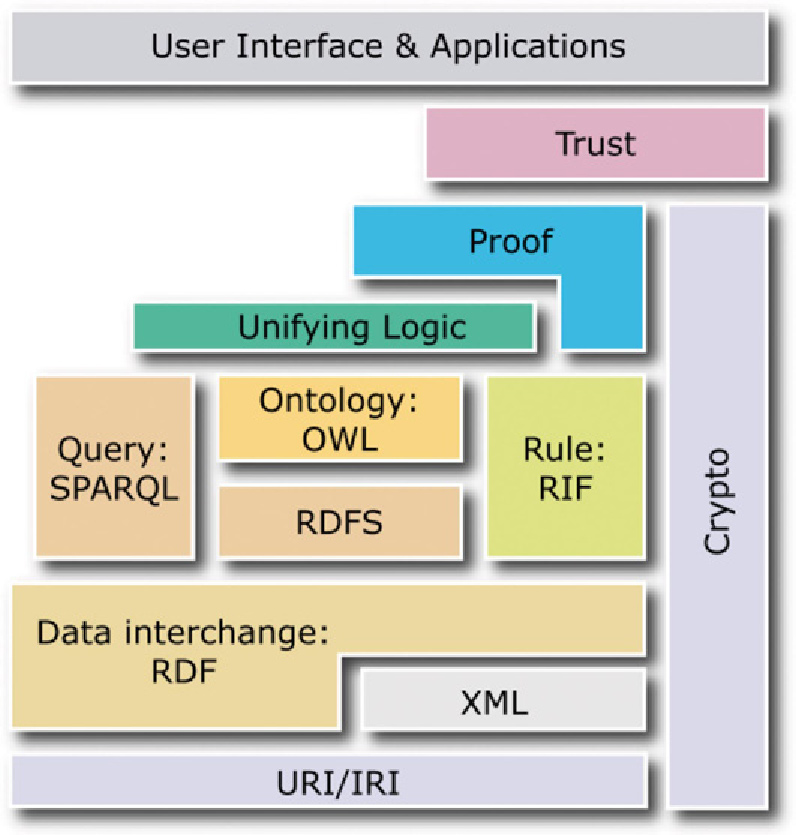
\includegraphics[width=7cm]{./assets/img/semantic_web_cake.jpg}
	\caption{The Semantic Web Cake}
	\label{fig:semantic_web_cake}
	\vspace{0.5cm}
\end{figure}

\section{RDF}

The Resource Description Framework, from now on RDF, is a data representation model that was defined in 1996 and adopted as a W3C recommendation in 1999. Originally, RDF was designed as a metadata data model, but later it has come to be used as a general method for conceptual description or modeling of information that is implemented in Web resources. Today, RDF has become an open-world framework that allows everyone to make statements about any resource. Hence, its goal is to allow the description of the resources that are uniquely identified in the Web by \textit{Internationalized Resource Identifiers}, from now on IRIs.

RDF plays a very important role in the Web of Data and the Semantic Web, which are extensions of the original World Wide Web, and consequently in the Big Data phenomenon. It has a simple data model that is easy for applications to process and manipulate. The data model is independent of any specific serialization syntax.

Any expression in RDF is a triple composed by a subject, a predicate and an object. A set of such triples is called RDF graph, since a triple can be illustrated by two nodes connected by an arc, as shown in \figurename~\ref{fig:rdf_triple}.

\begin{figure}
	\centering
	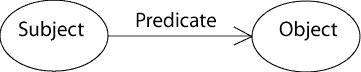
\includegraphics[width=7cm]{./assets/img/rdf_triple.png}
	\caption{Illustration of an RDF triple}
	\label{fig:rdf_triple}
	\vspace{0.5cm}
\end{figure}

In order to provide the signature of an RDF triple, we consider three disjointed sets: \\

\begin{itemize}
	\begin{minipage}{0.92\textwidth}
		\item $I$ a set of IRIs \\
	\end{minipage} \\
	\begin{minipage}{0.92\textwidth}
		\item $B$ a set of blank nodes just corresponding to nodes in an RDF graph which do not have intrinsic names \\
	\end{minipage} \\
	\begin{minipage}{0.92\textwidth}
		\item $L$ a set of literals where a literal is a lexical form and a datatype IRI, with a language tag in addition if the datatype IRI is \href{http://www.w3.org/1999/02/22-rdf-syntax-ns\#langString}{http://www.w3.org/1999/02/22-rdf-syntax-ns\#langString}. Literals are used for values such as strings, numbers and dates \\
	\end{minipage}
\end{itemize}

An RDF triple $T$ is then represented in form of: $T = (I \cup B) \times (I) \times (I \cup B \cup L)$. This indicates that a subject could be a IRI or a blank node, a predicate could only be a IRI and a object could be a IRI, a blank node or a literal.
Each triple represents a relationship between the subject and the object linked. The direction of the arc is significant: it always points toward the object.

Since RDF works on the Web, RDF data can originate from multiple sources. This implies a merging task whenever there are at least two sources. Interestingly, the merging phase is not a problem, because merging two or more sources means merging set of triples. Instead, the main problem that could arise is the identification of common resources among multiple sources, for instance blank nodes. But since RDF uses IRIs, every entity or node is uniquely identified across the Web.

Here it is possible to get a glimpse about the potential of RDF: any two data source on the Web can refer to the same resource and add extra information just by using the same IRI.
Obviously, IRIs also solve the problem of disambiguation, since the name that is used to describe that resource is only the final part of the IRI. The RDF standard provides the specific namespace often referred to with the \texttt{rdf} prefix name: \href{http://www.w3.org/1999/02/22-rdf-syntax-ns}{\texttt{<http://www.w3.org/1999/02/22-rdf-syntax-ns>}}.

\subsection{RDF/XML}

\textit{RDF/XML} is a syntax recommended by the W3C to express, then to serialize, an RDF graph as an XML document\cite{rdf_xml_w3c}. Briefly, any resource can be represented using an \texttt{rdf:Description} XML element, specifying its \texttt{rdf:about} attribute using an URI. Since the same element, i.e a subject, can have multiple characteristics, the nested structure of XML can be used to add them to the given subject. To specify the type of the resource represented, the \texttt{rdf:type} attribute has to be added as nested element in combination with the \texttt{rdf:resource}. See below for an example: \\

\begin{minipage}{0.92\textwidth}
	\lstset{language=xml}
	\begin{lstlisting}
<?xml version``1.0'' encoding=``UTF-8'' ?>
<rdf:RDF
    xmlns:rdf=``http://www.w3.org/1999/02/22-rdf-syntax-ns#''
    xmlns:ub=``http://swat.cse.lehigh.edu/onto/univ-bench.owl#''
> 

    <rdf:Description rdf:about=``http://www.University0.edu''>
        <rdf:type rdf:resource=``http://swat.cse.lehigh.edu/onto/univ-bench.owl#University''>
        <ub:name>University0</ub:name>
    </rdf:Description>
    
    <rdf:Description rdf:about=``http://www.Department0.University0.edu''>
        <rdf:type rdf:resource=``http://swat.cse.lehigh.edu/onto/univ-bench.owl#Department''>
        <ub:name>Department0</ub:name>
        <ub:subOrganizationOf>
            <ub:University rdf:about=``http://www.University0.edu'' />
        </ub:subOrganizationOf>
    </rdf:Description>
    
</rdf:RDF>
                \end{lstlisting}
\end{minipage} \\
\\

To make the definition of an element and its type easier and more concise, RDF/XML allows a shorter expression to combine the \texttt{rdf:Description} element and its \texttt{rdf:type} attribute by replacing them with an element directly named with the namespaced element corresponding to the RDF IRI of the \texttt{rdf:resource} attribute. A shorter way to declare the previous example is shown here: \\

\begin{minipage}{0.92\textwidth}
	\lstset{language=xml}
	\begin{lstlisting}
<?xml version=``1.0'' encoding=``UTF-8'' ?>
<rdf:RDF
    xmlns:rdf=``http://www.w3.org/1999/02/22-rdf-syntax-ns#''
    xmlns:ub=``http://swat.cse.lehigh.edu/onto/univ-bench.owl#''
> 

<ub:University rdf:about=``http://www.University0.edu''>
    <ub:name>University0</ub:name>
</ub:University>

<ub:Department rdf:about=``http://www.Department0.University0.edu''>
    <ub:name>Department0</ub:name>
    <ub:subOrganizationOf>
        <ub:University rdf:about=``http://www.University0.edu'' />
    </ub:subOrganizationOf>
</ub:Department>

</rdf:RDF>
                \end{lstlisting}
\end{minipage} \\
\\

Moreover, any predicate having a literal value can be expressed as an XML attribute of the corresponding subject element. The previous example code can thus be shortened even further as follows: \\

\begin{minipage}{0.92\textwidth}
	\lstset{language=xml}
	\begin{lstlisting}
<?xml version=``1.0'' encoding=``UTF-8'' ?>
<rdf:RDF
    xmlns:rdf=``http://www.w3.org/1999/02/22-rdf-syntax-ns#''
    xmlns:ub=``http://swat.cse.lehigh.edu/onto/univ-bench.owl#''
> 

<ub:University rdf:about=``http://www.University0.edu'' ub:name=``University0'' />
<ub:Department rdf:about=``http://www.Department0.University0.edu'' ub:name=``Department0''>
    <ub:subOrganizationOf>
        <ub:University rdf:about=``http://www.University0.edu'' />
    </ub:subOrganizationOf>
</ub:Department>

</rdf:RDF>
                \end{lstlisting}
\end{minipage} \\
\\

\subsection{N-Triples}

\textit{N-Triples} is a line-based, plain text format for encoding an RDF graph, and it is the simplest form of textual representation for RDF data. Its strength is also its greatest weakness: not allowing abbreviations makes N-Triples very human-readable but space-consuming and quite redundant. The triples are given in subject, predicate, and object order as three complete UIIs separated by spaces and encompassed by angle brackets, \texttt{<} and \texttt{>}. Each triple takes a single line ended by a period (\texttt{.}). Here it follows the translation to N-Triples format\footnote{Due to text-wrapping and to the meager page width, to facilitate the reading, triples are separated by a blank line and each triple takes 3 lines. Furthermore, the subject is colored in green, the predicate in blue and the object in violet} of the previous lines: \\

\begin{minipage}{0.92\textwidth}
	\begin{lstlisting}
<<@\textcolor{green}{http://www.University0.edu}@>> <@\\@> <<@\textcolor{blue}{http://www.w3.org/1999/02/22-rdf-syntax-ns\#type}@>> <@\\@> <<@\textcolor{violet}{http://swat.cse.lehigh.edu/onto/univ-bench.owl\#University}@>> . <@\\@>
<<@\textcolor{green}{http://www.University0.edu}@>> <@\\@> <<@\textcolor{blue}{http://swat.cse.lehigh.edu/onto/univ-bench.owl\#name}@>> <@\\@> <@\textcolor{violet}{``University0''}@> . <@\\@>
<<@\textcolor{green}{http://www.Department0.University0.edu}@>> <@\\@> <<@\textcolor{blue}{http://www.w3.org/1999/02/22-rdf-syntax-ns\#type}@>> <@\\@> <<@\textcolor{violet}{http://swat.cse.lehigh.edu/onto/univ-bench.owl\#Department}@>> . <@\\@>
<<@\textcolor{green}{http://www.Department0.University0.edu}@>> <@\\@> <<@\textcolor{blue}{http://swat.cse.lehigh.edu/onto/univ-bench.owl\#name}@>> <@\\@> <@\textcolor{violet}{``Department0''}@> .<@\\@>
<<@\textcolor{green}{http://www.Department0.University0.edu}@>> <@\\@> <<@\textcolor{blue}{http://swat.cse.lehigh.edu/onto/univ-bench.owl\#subOrganizationOf}@>> <@\\@> <<@\textcolor{violet}{http://www.University0.edu}@>> .
                \end{lstlisting}
\end{minipage} \\
\\

\subsection{Turtle}

\label{subsection:turtle}

\textit{Turtle}, the Terse RDF Triple Language, is becoming increasingly popular and it is now a W3C recommendation. In Turtle, as a predicate, \texttt{a} is equivalent to the complete IRI corresponding to \texttt{rdf:type}.

The notation is very similar to N-triples with a few differences. Aside from the fact that surrounding parentheses have been removed and IRIs can be abbreviated by prefixed names, the main syntactic difference is an abbreviated syntax for statements that share a predicate and/or an object: \\

\begin{itemize}
	\begin{minipage}{0.92\textwidth}
		\item
		``\texttt{subject predicate1 x ; predicate2 y .}'' stands for ``\texttt{subject predicate1 x . subject predicate2 y .}'' \\
	\end{minipage} \\
	\begin{minipage}{0.92\textwidth}
		\item
		``\texttt{subject predicate x , y .}'' stands for ``\texttt{subject predicate x . subject predicate y .}'' \\
	\end{minipage}
\end{itemize}

Here it follows the translation to Turtle format of the previous example: \\

\begin{minipage}{0.92\textwidth}
	\lstset{language=turtle}
	\begin{lstlisting}
@prefix ub: <http://swat.cse.lehigh.edu/onto/univ-bench.owl#>

<http://www.University0.edu>    a               ub:University ;
                                            ub:name      ``University0'' .
                                
<http://www.Department0.University0.edu>    a                               ub:Department ;
                                                              ub:name                      ``Department0'' ;
                                                              ub:subOrganizationOf     <http://www.University0.edu> .
                \end{lstlisting}
\end{minipage} \\
\\

\section{SPARQL}

\textit{SPARQL} is the standard query language and protocol for Linked Open Data and RDF databases. It enables users to query information from database or any data source that can be mapped to RDF. The SPARQL standard is designed and endorsed by the W3C to help users and developers focus on what they want to know, and not on how the database is organized.
The basic syntax of a SPARQL is very similar to a simple SQL query with \texttt{SELECT}-\texttt{FROM}-\texttt{WHERE} clauses, but the query processing is quite different. While most of the time SQL relies on joins between tables, SPARQL execution consists of navigating RDF graphs, then moving from node to node via edges until the desired node is reached. In fact, the execution of SPARQL queries is based on graph pattern matching between the graph of the \texttt{WHERE} clause and the RDF graph to be queried.

In contrast to SQL, SPARQL queries are not limited to working in just one database, but federated queries accessing multiple data stores (endpoints) are supported. This is technically feasible because SPARQL is more than just a query language. Indeed, it is also an HTTP-based transport protocol that can access any SPARQL endpoint through a standardized transport layer.

\subsection{Syntax}

A SPARQL query consists of a set of triple patterns specified in the \texttt{WHERE} clause, where each element, i.e. subject, predicate, and object, can be a variable (wildcard). Then, solutions to the variables are found by matching the pattern in the query with the triples in the data set. A variable is specified using a question mark (\texttt{?}) followed by its name and it can be used in more than a triple.
The clauses are expressed in Turtle (see Subsection \ref{subsection:turtle}), since it allows a short textual representation.

SPARQL has four types of queries: \\

\begin{enumerate}
	\begin{minipage}{0.92\textwidth}
		\item
		\texttt{ASK}: returns a \texttt{Boolean} value indicating whether a query pattern has a solution or not \\
	\end{minipage} \\
	\begin{minipage}{0.92\textwidth}
		\item
		\texttt{SELECT}: returns the variables solution and their bindings directly  in a tabular form. It supports many of the classic SQL options such as \texttt{LIMIT}, \texttt{DISTINCT}, \texttt{OFFSET}, \texttt{ORDER BY}, \texttt{GROUP BY} and \texttt{HAVING} \\
	\end{minipage} \\
	\begin{minipage}{0.92\textwidth}
		\item
		\texttt{CONSTRUCT}: returns a single RDF graph specified by a graph template, using each query solution, substituting the variables in these matches, and combining the triples into a single RDF graph by set union \\
	\end{minipage} \\
	\begin{minipage}{0.92\textwidth}
		\item
		\texttt{DESCRIBE}: asks for any RDF information related to some specific variables of the result template. It is usually used to discover resources without knowing their schema \\
	\end{minipage}
\end{enumerate}

Here follows an example for each type of SPARQL query\footnote{In order not to be redundant, prefixes have been omitted. The prefixes common to all queries are as follows:
	\vspace{0.1cm} \\
	\hspace*{0.8cm}\lstinline[language=sql]{PREFIX rdf: <http://www.w3.org/1999/02/22-rdf-syntax-ns#>} \\
	\hspace*{0.8cm}\lstinline[language=sql]{PREFIX ub: <http://www.lehigh.edu/~zhp2/2004/0401/univ-bench.owl#>} \\
}: \\

\begin{enumerate}
	\begin{minipage}{0.92\textwidth}
		\item
		\lstset{language=sql}
		\begin{lstlisting}
ASK {
    ?X rdf:type ub:GraduateStudent
}
                    \end{lstlisting}
	\end{minipage} \\
	\begin{minipage}{0.92\textwidth}
		\item
		\lstset{language=sql}
		\begin{lstlisting}
SELECT ?X
WHERE {
    ?X rdf:type ub:UndergraduateStudent
}
                    \end{lstlisting}
	\end{minipage} \\
	\begin{minipage}{0.92\textwidth}
		\item
		\lstset{language=sql}
		\begin{lstlisting}
PREFIX foaf: <http://xmlns.com/foaf/spec/>
CONSTRUCT {
    ?x foaf:name ?y
} WHERE { 
    ?x ub:name ?y
}
                    \end{lstlisting}
	\end{minipage} \\
	\begin{minipage}{0.92\textwidth}
		\item
		\lstset{language=sql}
		\begin{lstlisting}
DESCRIBE ?x
WHERE {
    ?X rdf:type ub:UndergraduateStudent .
    ?X ub:memberOf <http://www.Department0.University0.edu>
}
                    \end{lstlisting}
	\end{minipage} \\
\end{enumerate}

SPARQL also provides the following additional keywords: \\

\begin{itemize}
	\begin{minipage}{0.92\textwidth}
		\item \texttt{FILTER} restricts the solutions of a graph pattern match according to a given expression. Its use is similar to the SQL's \texttt{WHERE} clause. \\
	\end{minipage} \\

	\begin{minipage}{0.92\textwidth}
		\item \texttt{OPTIONAL} provides the possibility to not reject the solution because some parts of the query pattern do not match. Indeed, if the optional part does not match, it creates no bindings but it does not eliminate the solution. \\
	\end{minipage} \\
	\begin{minipage}{0.92\textwidth}
		\item \texttt{UNION} allows to combine several graphs, then to provide different alternatives. Hence, if more than one of the alternatives matches, all the possible pattern solutions are returned. \\
	\end{minipage} \\
	\begin{minipage}{0.92\textwidth}
		\item \texttt{FROM} allows to retrieve data and to consider more than one data set, i.e. graph. Then all data sets declared will be considered as just one. \\
	\end{minipage} \\
	\begin{minipage}{0.92\textwidth}
		\item \texttt{SERVICE} provides a way to remotely execute a query on a SPARQL endpoint, that is a web service allowing SPARQL queries, then to perform federated queries. Federated queries allows to take a query and provide solutions based on information from many different sources \\
	\end{minipage}
\end{itemize}

Lastly, the SPARQL 1.1 Update provides new two categories of operations: graph update, e.g. \texttt{INSERT}, \texttt{DELETE}, \texttt{LOAD}, \texttt{CLEAR} et cetera, and graph management, e.g., \texttt{CREATE GRAPH} and \texttt{DROP GRAPH}.

\section{Ontologies}

Delving into ontologies and related languages of ontologies is far from the goal of this work, but it was deemed important to at least give a taste of what an ontology is after the RDF presentation that has been addressed in the previous two sections, since they provide semantic interpretations to RDF facts.

So far the values of subjects, properties, and objects have been specified without considering what their values represent. To solve this problem, ontologies come to the rescue. As Thomas Gruber, the co-founder of Siri, Apple's intelligent personal assistant, claimed in 1993, ``\textit{an ontology is a specification of a conceptualization}''. In other words, it aims to conceptualize a domain by strictly specifying the entities it contains and all the relationships that might exist between them.

In the Semantic Web context, there are a large number of ontology languages, such as RDFS and the OWL2 family, and the main difference lies in their expressiveness. \figurename~\ref{fig:ontologies_languages} describes it.

\begin{figure}
	\centering
	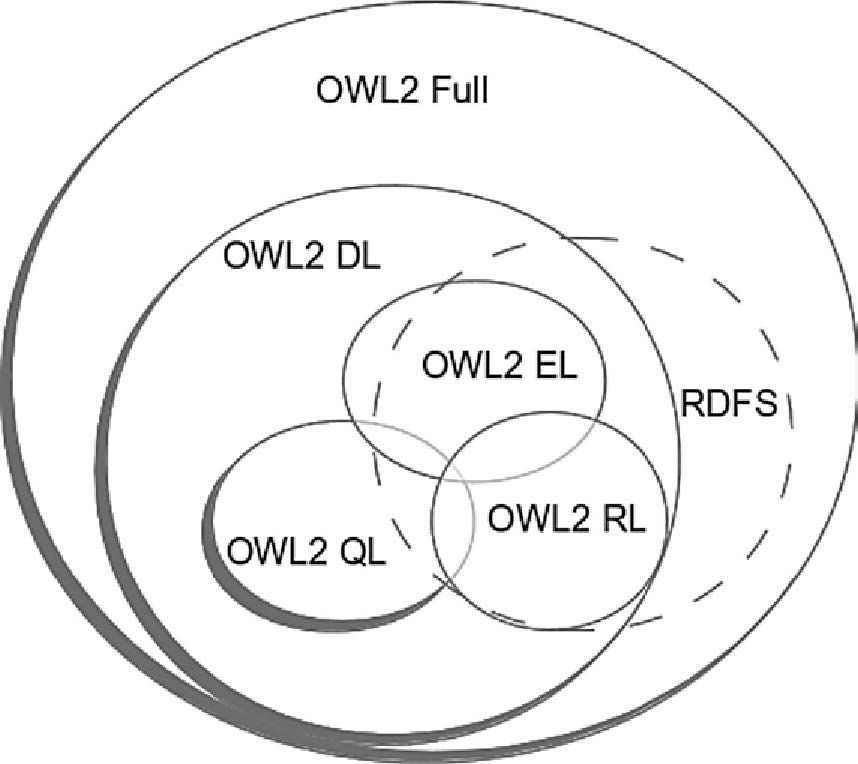
\includegraphics[width=6cm]{./assets/img/ontologies_languages.jpg}
	\caption{Expressiveness of OWL2 and RDFS ontology languages}
	\label{fig:ontologies_languages}
	\vspace{0.5cm}
\end{figure}

What is important is that ontologies provide a mechanism to describe groups of related resources and their relationships defining \textit{classes}, \textit{properties}, \textit{instances} and \textit{meta-descriptions} with high accuracy. Therefore, since ontologies carry structure and hierarchies, they make inference about data possible. For example, a query might ask to retrieve all the students of a university, but the  students are stored as instances either of the \texttt{UndergraduateStudent} or \texttt{GraduateStudent} classes. While in a SQL environment this problem would lead to a rewriting query process, several current SPARQL engines and RDF stores support rule based inference using ontologies.

\section{RDF storage techniques}

Because of its recent establishment, the RDF data model is still lacking in terms of storage. In fact, the search for an efficient storage backend is still considered an open problem.

Because since 1999, the year of the first W3C recommendation, several systems have been introduced, it is useful to try to classify them. First of all, it is possible to distinguish between \textit{native} and \textit{non-native} approaches. The former are those solutions that are implementing their own brand-new storage backend. The latter are those solutions that are trying to adopt existing database management system to the RDF data model.

\figurename~\ref{fig:rdf_storage_classification} tries to classify the several main techniques of storage currently used to deal with the RDF data model.

\begin{figure}
	\centering
	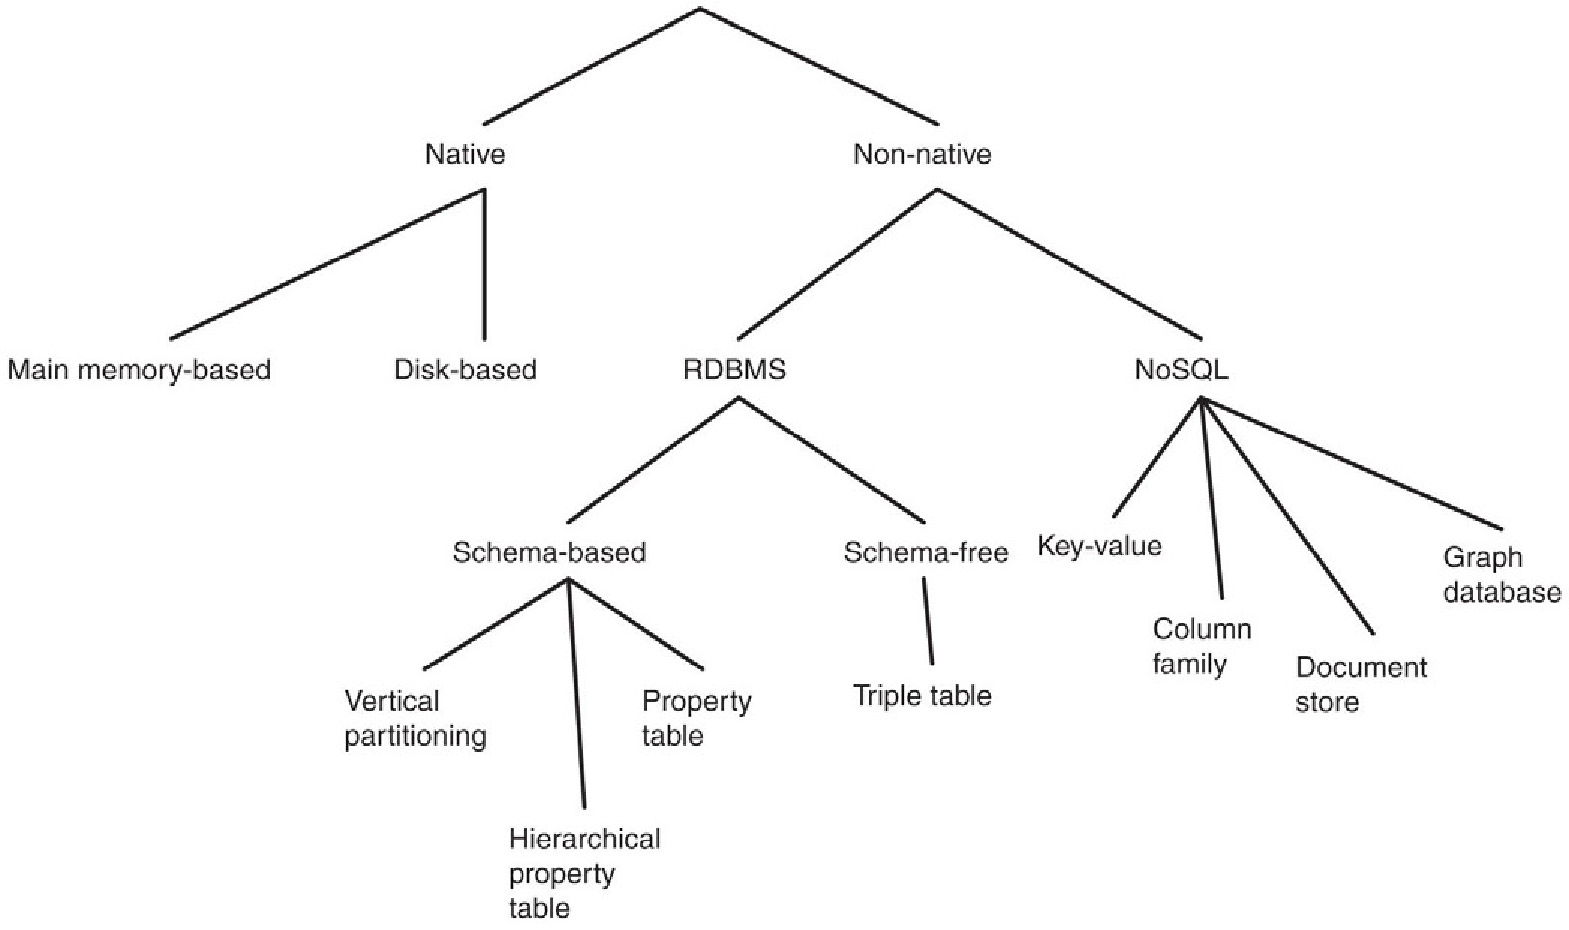
\includegraphics[width=12cm]{./assets/img/rdf_storage_classification.jpg}
	\caption{RDF storage techniques classification}
	\label{fig:rdf_storage_classification}
	\vspace{0.5cm}
\end{figure}

Describing the several techniques and the many existing systems is out of the goal of this work since it would require a chapter just to describe the main ones. Thus, only the concepts useful to the comprehension of this work are about to be deepened. To have a wider overview, please refer to the book written by the supervisor\cite{rdf_database_system}.

\subsection{Non-native approaches}

The non-native approaches benefits from dozens of years of research and development since they use database management systems, from now on DBMS, to store RDF data. These can be further divided into schema-free and schema-based approaches. In the former, just a single 3-column table is created and it stores all the triples. In the latter, the RDF triples are splitted into different tables.

\subsubsection{Schema-free approaches}

As already claimed, in schema-free approaches just one large table, called \textit{triples table}, is created. Then, each\texttt{ [subject}, \texttt{predicate}, \texttt{object] }RDF statement is stored as a row of a three-column table. Since all triples are stored in just one table, is very important to arrange them in an appropriate way to avoid slow queries, which are more than a considerable risk in such systems. In addition, complex queries with multiple triple patterns may perform poorly because they require many self-joins on this single large table. Table \ref{table:triples_example} shows an example of triples table\footnote{In the URLs \texttt{ http://www.} is omitted}.

\begin{table}
	\begin{center}
		\begin{tabular}{ | c | c | c | }
			\hline
			\textbf{subject}                                                 & \textbf{predicate} & \textbf{object} \\
			\hline
			\texttt{\scriptsize{Department0.University0.edu}}                &
			\texttt{\scriptsize{rdf:type}}                                   &
			\texttt{\scriptsize{ub:Department}}                                                                     \\
			\texttt{\scriptsize{Department0.University0.edu}}                &
			\texttt{\scriptsize{ub:name}}                                    &
			\texttt{\scriptsize{``Department0''}}                                                                   \\
			\texttt{\scriptsize{Department0.University0.edu}}                &
			\texttt{\scriptsize{ub:subOrganizationOf}}                       &
			\texttt{\scriptsize{University0.edu}}                                                                   \\
			\texttt{\scriptsize{University0.edu}}                            &
			\texttt{\scriptsize{rdf:type}}                                   &
			\texttt{\scriptsize{ub:University}}                                                                     \\
			\texttt{\scriptsize{Department0.University0.edu/FullProfessor0}} &
			\texttt{\scriptsize{rdf:type}}                                   &
			\texttt{\scriptsize{ub:FullProfessor}}                                                                  \\
			\texttt{\scriptsize{Department0.University0.edu/FullProfessor0}} &
			\texttt{\scriptsize{ub:name}}                                    &
			\texttt{\scriptsize{``FullProfessor0''}}                                                                \\
			\texttt{\scriptsize{Department0.University0.edu/FullProfessor0}} &
			\texttt{\scriptsize{ub:undergraduateDegreeFrom}}                 &
			\texttt{\scriptsize{University1.edu}}                                                                   \\
			\texttt{\scriptsize{University1.edu}}                            &
			\texttt{\scriptsize{rdf:type}}                                   &
			\texttt{\scriptsize{ub:University}}                                                                     \\
			\texttt{\scriptsize{Department0.University0.edu/FullProfessor0}} &
			\texttt{\scriptsize{ub:mastersDegreeFrom}}                       &
			\texttt{\scriptsize{ University2.edu}}                                                                  \\
			\texttt{\scriptsize{University2.edu}}                            &
			\texttt{\scriptsize{rdf:type}}                                   &
			\texttt{\scriptsize{ub:University}}                                                                     \\
			\hline
		\end{tabular}
	\end{center}
	\caption{Example of triples table\\}
	\label{table:triples_example}
	\vspace{0.5cm}
\end{table}

\section{Cloud computing and Big Data}

Without a doubt, over the past few years the Big Data phenomenon and the cloud computing new technologies brought innovation providing new paradigms to improve and/or enable research and decision-support applications that few years ago were not feasible due to elevated costs and the impossibility to collect such a large amount of data. While Big Data and its techniques provided the possibility to collect, store, process and serve the data, cloud computing gives a fundamental support to address the challenges with shared computing resource\cite{cloud_computing_and_big_data}. It is a matter of fact that nowadays Cloud Computing and Big Data seem to be indissoluble.

The Big Data definition is often associated with the so-called 3 Vs: Volume, Velocity and Variety. These three Vs summarize the key aspects in this context well enough: \\

\begin{itemize}
	\begin{minipage}{0.92\textwidth}
		\item Volume emphasises that the size of the data cannot be stored and/or processed with an everyday and usual machine, but it requires a powerful server or a cluster of machines \\
	\end{minipage} \\
	\begin{minipage}{0.92\textwidth}
		\item Velocity indicates the speed with which the data arrive and therefore should be processed. It may require new paradigms to allow algorithms to run in clusters, e.g. a stream processing engine such as Flink or Spark \\
	\end{minipage} \\
	\begin{minipage}{0.92\textwidth}
		\item Variety concerns the format in which the data are presented. Three formats are possible: structured, semi-structured and unstructured. Data stored in relational RDBMS are surely an example of structured data, while examples of semi-structured formats are XML, JSON and RDF files. Unstructured data are those data poorly characterized such as images and textual documents.\\
	\end{minipage}
\end{itemize}

As the amount of Web data increases every day, there is a need for technologies and techniques to handle the enormous amount of Semantic Web that arise. These technologies must provide scalable and high performance storage solutions for these Web data. In this context, Cloud computing providers such as Amazon Web services\cite{aws}, from now on AWS, Microsoft Azure\cite{azure} and Google Cloud Platform\cite{google_cloud}, come into play by offering cloud computing capabilities.

Cloud computing is the on-demand availability of computer system resources, in particular computing power and data storage, based on the sharing of resources. Indeed, the largest cloud providers, predominant today, usually have data centers distributed over several locations. They usually adopt the ``pay-as-you-go'' model where users pay just for services and resources they use. Thus, among the advantages of cloud platforms there are surely their ease of use that avoids tedious management, the ease of scaling systems, both horizontally and vertically, and their low costs.

Since an increasing number of organizations and communities keep their data available in the RDF format, there is the need of an efficient RDF storage system for querying these data in a scalable and efficient way, and cloud solutions might fit well.

\subsection{Apache Hadoop and Apache Spark}

Among distributed systems, Apache Hadoop in combination with Apache Spark have been the most used for some time now. The Apache Hadoop project develops open-source softwares for reliable, scalable, distributed computing. Indeed, the Apache Hadoop software library is a framework that allows distributed processing of large data sets across clusters of computers using simple programming models. It has been designed to scale up from single servers to thousands of machines, each offering local computation and storage, using a shared-nothing architecture. The library itself is designed to detect and handle failures at the application layer, so to deliver a highly-available service on top of a cluster of computers, each of which may be prone to failures\cite{apache_hadoop}. The Hadoop project includes the following modules: \\

\begin{itemize}
	\begin{minipage}{0.92\textwidth}
		\item The Hadoop Common utilities that support the other Hadoop modules \\
	\end{minipage} \\
	\begin{minipage}{0.92\textwidth}
		\item The Hadoop Distributed File System\cite{hdfs}, from now on HDFS, that provides high-throughput access to application data \\
	\end{minipage} \\
	\begin{minipage}{0.92\textwidth}
		\item The Hadoop YARN (Yet Another Resource Negotiator) framework to handle job scheduling and cluster resource management \\
	\end{minipage} \\
	\begin{minipage}{0.92\textwidth}
		\item The Hadoop MapReduce\cite{mapreduce} system for parallel processing of large data sets. \\
	\end{minipage}
\end{itemize}

On the other hand, Apache Spark is a unified analytics engine for large-scale data processing. It provides high-level APIs in Java, Scala, Python and R. It also supports a rich set of higher-level tools including Spark SQL and structured data processing. Furthermore, it features an optimised engine that supports general graph processing\cite{apache_spark}.

The main abstraction Spark provides is the Resilient Distributed Data set (RDD), which is a collection of elements distributed on a cluster of machines that can be managed in parallel and maintained in a fault-tolerant manner. \figurename~\ref{fig:spark_stack} shows a minimal representation of the Spark stack.

\begin{figure}
	\centering
	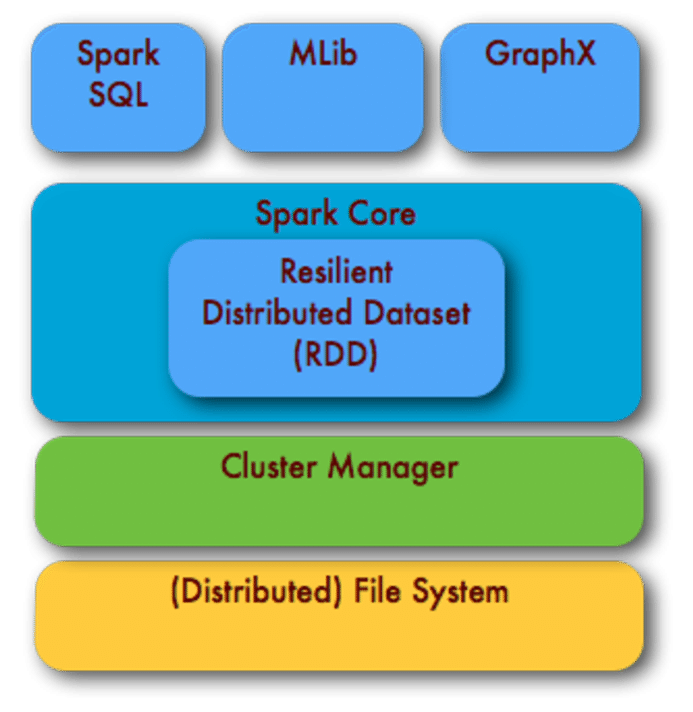
\includegraphics[width=5cm]{./assets/img/spark/apache_spark_stack.png}
	\caption{Apache Spark stack}
	\label{fig:spark_stack}
	\vspace{0.5cm}
\end{figure}

Spark applications run as independent sets of processes on a cluster, coordinated by the \texttt{SparkContext} object in the main program, called the driver program. More in detail, to run on a cluster, the \texttt{SparkContext} connects to several types of cluster managers, which allocate resources across applications. Once connected, Spark acquires executors on nodes in the cluster, which are processes that run computations and store data for applications. Next, it sends the application code to the executors. Finally, the \texttt{SparkContext} sends tasks to run to the executors\cite{apache_spark_architecture}. \figurename~\ref{fig:spark_architecture} shows a simplified representation of the Spark architecture.

\begin{figure}
	\centering
	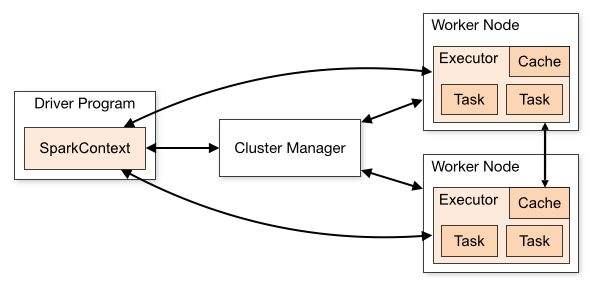
\includegraphics[width=11cm]{./assets/img/spark/apache_spark_architecture.png}
	\caption{Apache Spark architecture}
	\label{fig:spark_architecture}
	\vspace{0.5cm}
\end{figure}

\section{Columnar storage}

While a relational storage is optimized for storing rows of data and to access very quickly singular rows, typically for transactional applications, a columnar database is optimized for fast retrieval of columns of data, typically in analytical applications. The purpose of transactional data is to support day-to-day operations of the business and it is exceedingly valuable for that purpose. In contrast, analytical data is used for managerial analysis and decision making. Storing data in a columnar format allows to read, decompress, and process only those values that are required for the current query.

To give an example, while the row format is stored as \texttt{Row 1 > Row 2 > Row 3}, the columnar format is stored to disk as \texttt{Column 1 > Column 2 > Column 3}.
\figurename~\ref{fig:row_vs_column_storage} shows a very simplified table to highlight the differences between the two different storage techniques.

\begin{figure}
	\centering
	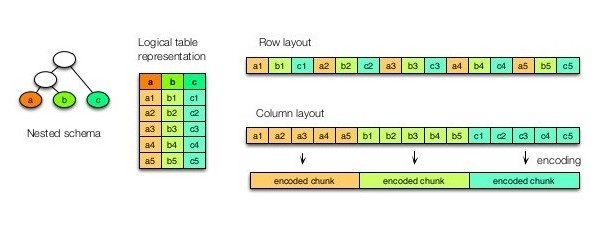
\includegraphics[width=12cm]{./assets/img/row_vs_column.jpg}
	\caption{Row vs column based storage}
	\label{fig:row_vs_column_storage}
	\vspace{0.5cm}
\end{figure}

Thus, when the goal is usually to recover the punctual data, e.g. all data of a row, row storage is undoubtedly the best solution. But, when the goal is to access large amounts of data stored in few columns to help the decision making process, so to access analytical data, e.g the average of a column, columnar storage is clearly a better solution. This happens because in a relational storage all rows must be read to extract just one column value, while in a columnar storage all data are read in one-shot because they are stored in contiguous blocks.

Hence, column-oriented storage for tables is an important factor in analytic query performance because it drastically reduces the overall disk I/O requirements and reduces the amount of data needed to be loaded from disk.
Furthermore, column-oriented databases are designed to scale-out using distributed clusters of low-cost hardware to increase throughput, making them ideal for data warehousing and Big Data processing.

Some of the most famous and used columnar storage formats are, in chronological order: ORC, Parquet, CarbonData and Arrow. All of these formats are supported by the \textit{Apache Software Foundation}\footnote{From this point onward, the term ``Apache'' will be omitted not to be redundant}. All formats are optimized for storage on Apache Hadoop, hence they enable scalability, parallel processing and provide some degrees of compression, that is a very important factor when using a non-free cloud provider.

Furthermore, Arrow is something more than just a columnar format. Indeed, it is a cross-language development platform for in-memory analytics\cite{arrow_homepage}. For this reason it can be used on top of other formats, such as Parquet.

\subsection{Glossary}

In order to facilitate the reader's understanding, some definitions of very common terms in the columnar storage context are provided below: \\

\begin{itemize}
	\begin{minipage}{0.92\textwidth}
		\item File: a HDFS file that must include the metadata for the file. It does not need to actually contain the data \\
	\end{minipage} \\
	\begin{minipage}{0.92\textwidth}
		\item Stripe: a collection of row groups \\
	\end{minipage} \\
	\begin{minipage}{0.92\textwidth}
		\item Row group: a logical horizontal partitioning of the data into rows. There is no physical structure that is guaranteed for a row group. It consists of a column chunk for each column in the data set \\
	\end{minipage} \\
	\begin{minipage}{0.92\textwidth}
		\item Column chunk: a chunk of the data for a particular column. It is contained in a particular row group and is guaranteed to be contiguous in the file \\
	\end{minipage} \\
	\begin{minipage}{0.92\textwidth}
		\item Page: column chunks are divided up into pages. A page is conceptually an indivisible unit, in terms of compression and encoding. Unless specified, there can be multiple page types that interleave in a column chunk \\
	\end{minipage}
\end{itemize}

Hierarchically summarised, a file consists of one or more row groups. A row group contains exactly one column chunk per column. Column chunks contain one or more pages.

\subsection{Apache CarbonData}

\textit{Apache CarbonData} is an indexed columnar binary data format for fast analytics on Big Data platforms\cite{carbondata_homepage}, such as Apache Hadoop and Apache Spark. It aims to take advantage of its advanced columnar storage index for fast interactive querying. To achieve this, it uses compression and encoding techniques to improve computational efficiency.

As pointed out by \figurename~\ref{fig:carbondata_homepage}, CarbonData enables users to access the whole data using a single copy. The challenge is then to answer efficiently all different types of queries: \\

\begin{itemize}
	\begin{minipage}{0.92\textwidth}
		\item OLAP (OnLine Analytical Processing) queries, which are complex queries that use large amounts of data. These queries are used to perform complex analysis of the data, typically in a data warehouse \\
	\end{minipage} \\
	\begin{minipage}{0.92\textwidth}
		\item Big scan and small scan queries, which are queries that require scans of larger or limited areas respectively \\
	\end{minipage} \\
	\begin{minipage}{0.92\textwidth}
		\item Point queries that consume a small portion of the big table \\
	\end{minipage}
\end{itemize}

\begin{figure}
	\centering
	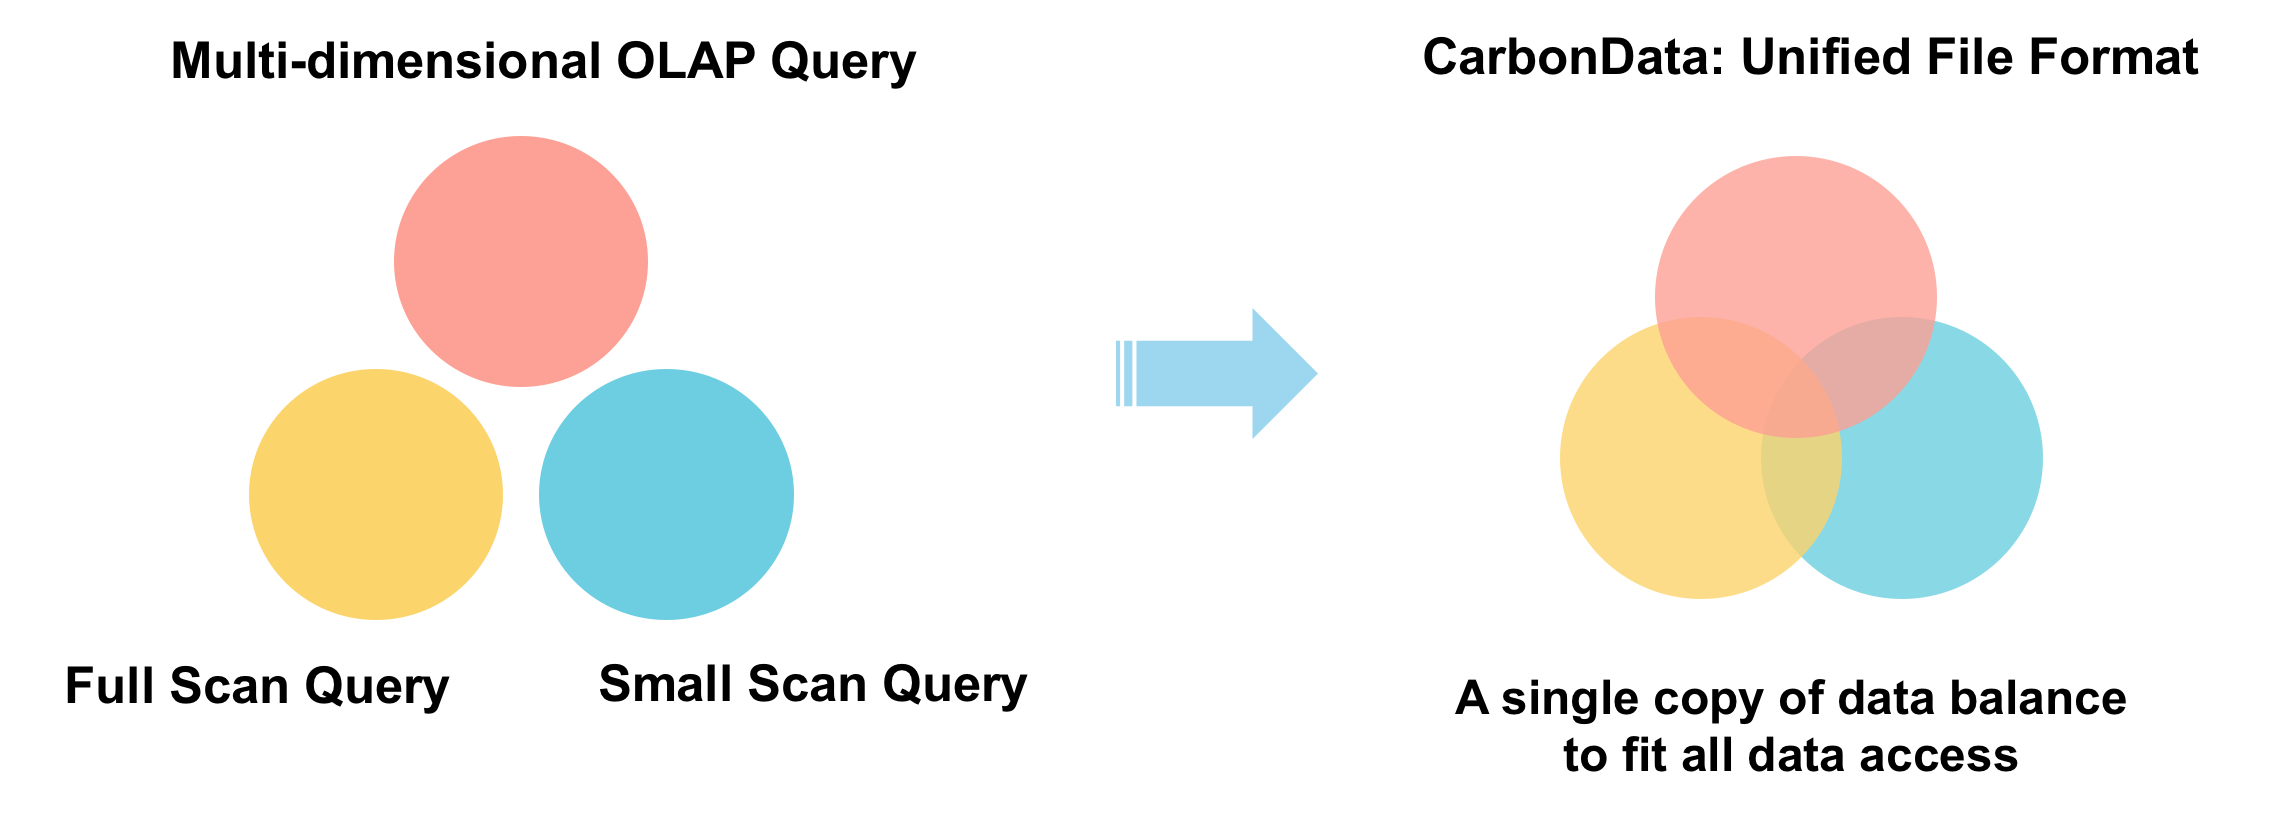
\includegraphics[width=12cm]{./assets/img/carbondata/carbondata.png}
	\caption{CarbonData unified file format}
	\label{fig:carbondata_homepage}
	\vspace{0.5cm}
\end{figure}

\begin{figure}
	\centering
	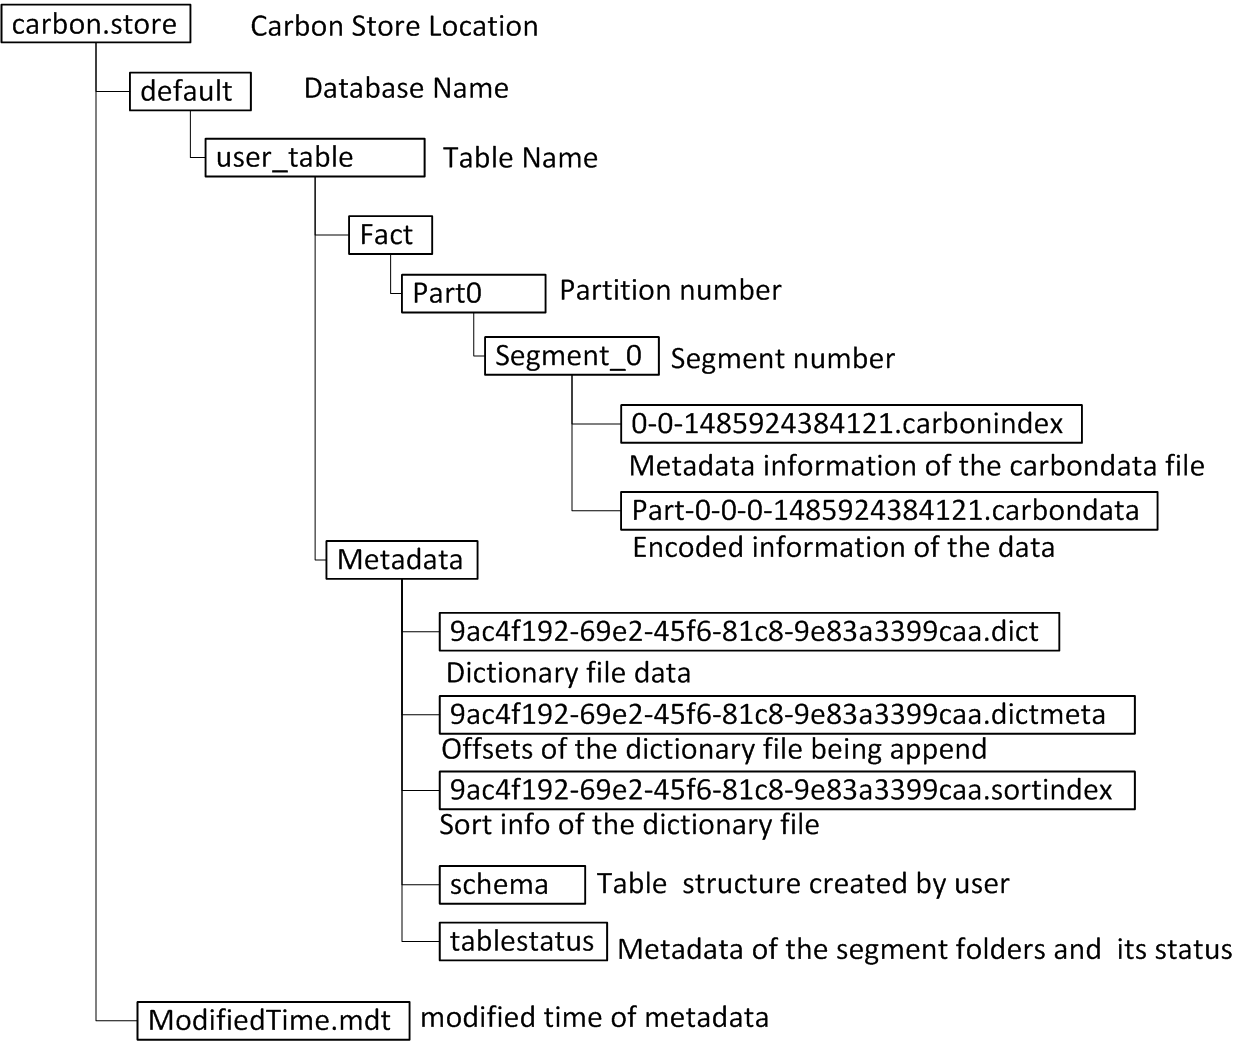
\includegraphics[width=13cm]{./assets/img/carbondata/carbondata_file_directory_structure.png}
	\caption{CarbonData file directory structure}
	\label{fig:carbondata_file_directory_structure}
	\vspace{0.5cm}
\end{figure}

The CarbonData files are stored in the location specified by the\texttt{ carbon.storelocation }configuration. \figurename~\ref{fig:carbondata_file_directory_structure} shows the file directory structure, that is the structure of the directory containing all the files related to the original file. More in details: \\

\begin{itemize}
	\begin{minipage}{0.92\textwidth}
		\item \texttt{ModifiedTime.mdt} records the timestamp of the metadata with the modification time attribute of the file. It is common to all databases and it is used to keep them updated \\
	\end{minipage} \\
	\begin{minipage}{0.92\textwidth}
		\item The database name is \texttt{default}, unless specified otherwise, and it contains the so-called \texttt{user\_table} \\
	\end{minipage} \\
	\begin{minipage}{0.92\textwidth}
		\item There are three types of metadata files. Indeed, the \texttt{Metadata} directory stores information about schema files, tablestatus and dictionary files \\
	\end{minipage} \\
	\begin{minipage}{0.92\textwidth}
		\item The data and index files are stored in the \texttt{Fact} directory. This folder contains the partitions identified by the number following the name \texttt{Part}. In turn, the partition folder contains the segments, identified by a number as well. Each segment folder contains then two types of files: \textit{CarbonData} and \textit{carbonindex}.\\
	\end{minipage}
\end{itemize}

Then, when a table is created, the \texttt{user\_table} directory and the schema file for recording the table structure are generated.

\begin{figure}
	\centering
	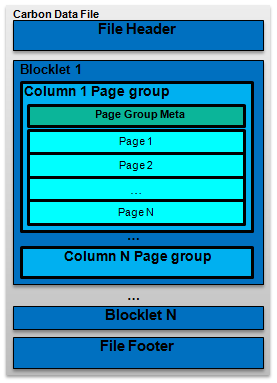
\includegraphics[width=6cm]{./assets/img/carbondata/carbondata_file_structure.png}
	\caption{CarbonData file structure}
	\label{fig:carbondata_file_structure}
	\vspace{0.5cm}
\end{figure}

CarbonData files have 3 main components: a header, a groups of data called blocklets and a footer. The header contains the CarbonData file version number, a list of column schema and the schema updating timestamp. The footer is used to build the indices in memory, which can be exploited for optimizing the scans and processing for all subsequent queries\cite{carbondata_structure}. \figurename~\ref{fig:carbondata_file_structure} shows the main structure of a CarbonData file. As already mentioned, a CarbonData file consists then of multiple blocklets. A blocklet is the data set inside the CarbonData file, whose size is usually 64MB.

There are three version of CarbonData file available, V1, V2 and V3, and they differ mainly for the blocklet structure. \figurename~\ref{fig:carbondata_file_v3} describes the structure of the most recent one.

\begin{figure}
	\centering
	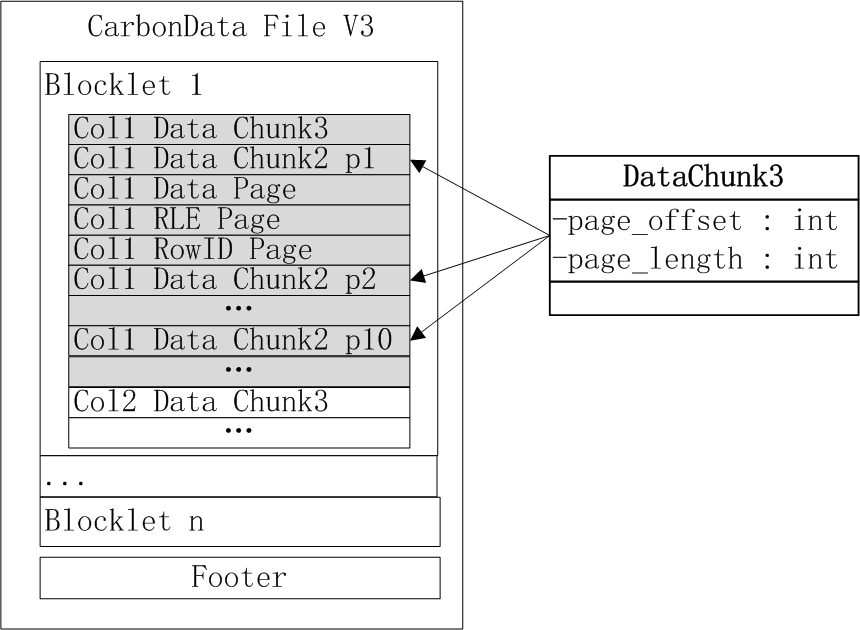
\includegraphics[width=11cm]{./assets/img/carbondata/carbondata_blocklet.png}
	\caption{CarbonData file V3}
	\label{fig:carbondata_file_v3}
	\vspace{0.5cm}
\end{figure}

The blocklet is composed of \texttt{ColumnChunks} of all columns. \texttt{ColumnChunk} consists of one or more \texttt{ColumnPages}. Each \texttt{ColumnPage} includes: \\

\begin{itemize}
	\begin{minipage}{0.92\textwidth}
		\item the data chunk header, which records the length information of all pages \\
	\end{minipage} \\
	\begin{minipage}{0.92\textwidth}
		\item the \texttt{Data Page}, which contains the encoded data \\
	\end{minipage} \\
	\begin{minipage}{0.92\textwidth}
		\item the \texttt{RLE page}, which contains some additional meta-information. It is used when the \texttt{Data Page} uses RLE encoding \\
	\end{minipage} \\
	\begin{minipage}{0.92\textwidth}
		\item the \texttt{rowID page}, which contains the mapping of the row id. It is used when the \texttt{Data Page} is stored in the form of an inverted index \\
	\end{minipage} \\
	\begin{minipage}{0.92\textwidth}
		\item a \texttt{BlockletMinMaxIndex} \\
	\end{minipage}
\end{itemize}

Since the header part records the length information of all the pages, the footer part only needs to record the offset and length of the ColumnChunk. Indeed, it contains all blocklet data distribution information and statistical related metadata information.

\figurename~\ref{fig:carbondata_footer_structure} shows the structure of the footer. It contains most of the information used to index the data. More in details, the CarbonData index is composed of multi-level indexes including multi-dimensional (B\textsuperscript{+}trees), min/max and inverted index. With \texttt{BlockletBtreeIndex}, the range of blocklets satisfying the conditions in each block are delineated, while \texttt{BlockletMinMaxIndex} is used to record the min/max value of all columns in the blocklet.

\begin{figure}
	\centering
	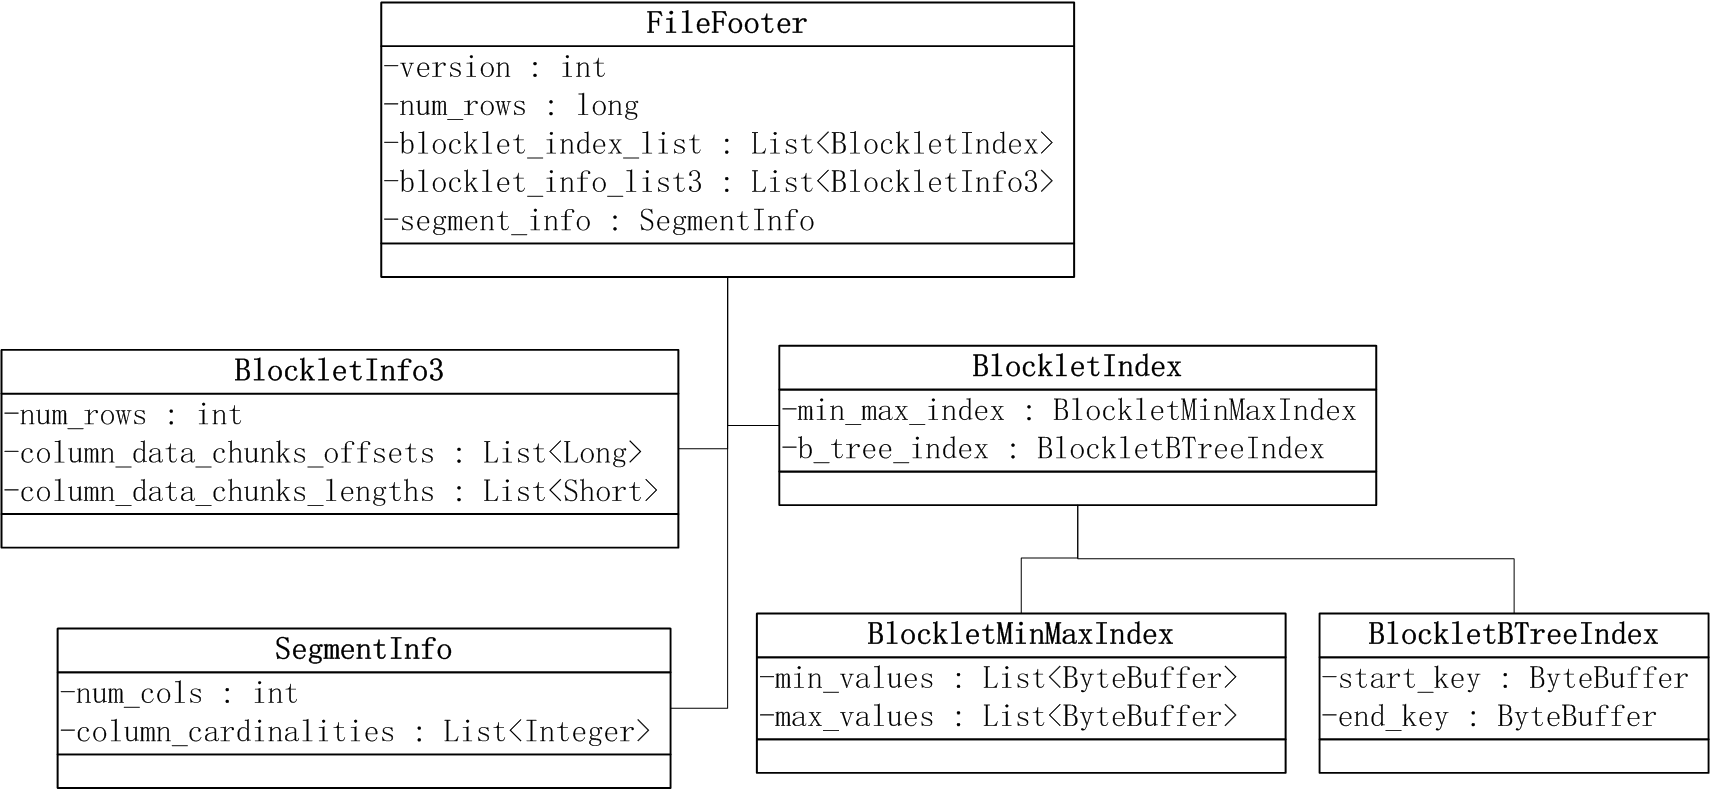
\includegraphics[width=13cm]{./assets/img/carbondata/carbondata_footer_structure.png}
	\caption{CarbonData footer structure}
	\label{fig:carbondata_footer_structure}
	\vspace{0.5cm}
\end{figure}

\subsection{Apache ORC}

The \textit{Optimized Row Columnar}, from now on ORC, is a self-describing binary type-aware columnar file format designed for Apache Hadoop workloads. It is optimized for large streaming reads, with integrated support for retrieving required rows quickly. Since ORC files are type-aware, the writer chooses the most appropriate encoding for the type and builds an internal index as the file is written. These indexes are then used to determine which stripes in a file need to be read for a particular query. The row indexes are used to narrow the search to a particular set of rows.

Usually, ORC files are divided into stripes that are 64 MB by default. The stripes in a file are independent. Within each stripe, the columns are separated from each other so the reader can read just the columns required\cite{orc_homepage}. As already specified, all ORC files are self-contained, i.e. it does not depend on the user’s environment to correctly interpret the file’s contents. To achieve this goal, every ORC file includes all of the type and encoding information for the objects stored.

ORC supports many primitive types, such as \texttt{boolean}, \texttt{int}, \texttt{float}, \texttt{string}, et cetera. But, it includes also more complex types such as structs, lists, maps, and unions. This is relevant because ORC files are logically sequences of identically typed objects.

Another important feature of ORC is its support for ACID transactions. But, as specified in the official documentation, although it supports ACID transactions, it is not designed to support OLTP requirements. ORC can support millions of rows updated per a transaction, but it cannot support millions of transactions per hour. Since HDFS is a write once file system and ORC is a write-once file format, edits are implemented using base files and delta files where insert, update, and delete operations are recorded. However, when deltas are too many or too large, merging and re-basing mechanisms are required and performed.

In order to provide light-weight compression techniques such as dictionary encoding, bit packing, delta encoding and run length encoding, ORC uses type specific readers and writers. This makes the resulting files considerably smaller. Additionally, ORC can apply generic compression algorithm such as Snappy\cite{google_snappy} on top of the light-weight compression for even smaller files.

ORC provides three level of indexes within each file: \\

\begin{itemize}
	\begin{minipage}{0.92\textwidth}
		\item File level indexes, which contain statistics about the values in each column across the entire file \\
	\end{minipage} \\
	\begin{minipage}{0.92\textwidth}
		\item Stripe level indexes, which contain statistics about the values in each column for each stripe \\
	\end{minipage} \\
	\begin{minipage}{0.92\textwidth}
		\item Row level indexes, which are light-weight indexes that contain statistics about the values in each column for each set of 10000 rows within a stripe and the position for seeking to the start of the row group. Moreover, row level indexes include both the minimum and maximum values for the entire file as well \\
	\end{minipage}
\end{itemize}

Beyond the statistics that record the count and, depending on the type, other useful fields such as min/max, the indexes may include Bloom filters, which provide a much more selective filter. Indeed, Bloom filters are used to speed up the process of finding equalities.

To easily determine which files need to be accessed and to avoid multiple passes during writing, the file and stripe level column statistics are in the file footer. Then, using pushdown filters, which are a way to enable the execution of certain filters at the data source before it is loaded to an executor process, the file reader can skip entire sets of rows that are not important for the current query\cite{orc_format}.

There have been two released ORC file versions: \\
\begin{itemize}
	\begin{minipage}{0.92\textwidth}
		\item ORC v0 was released in Hive 0.11 \\
	\end{minipage} \\
	\begin{minipage}{0.92\textwidth}
		\item ORC v1 was released in Hive 0.12 and ORC 1.x \\
	\end{minipage}
\end{itemize}
Furthermore, the \textit{Apache Software Foundation} is currently working on a new version of the file format: ORC v2\cite{orc_specification}.

\subsubsection{ORC v1 format}

\figurename~\ref{fig:orc_format} shows the overall structure of an ORC v1 file. The file can be broken down into three parts: header, body, and tail.

\begin{figure}
	\centering
	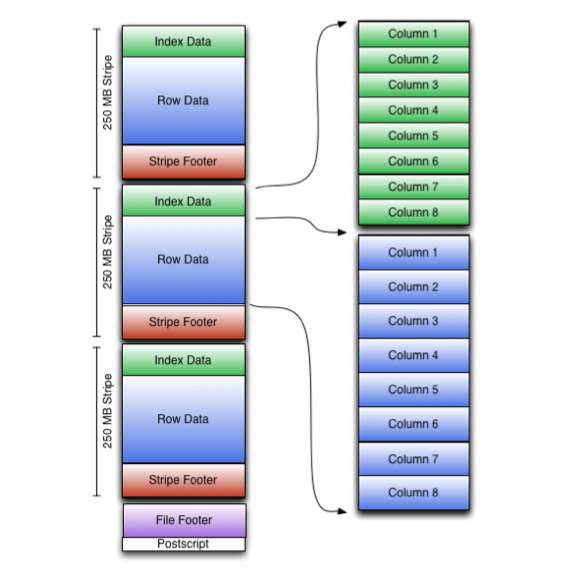
\includegraphics[width=11cm]{./assets/img/orc_format.png}
	\caption{ORC file format}
	\label{fig:orc_format}
	\vspace{0.5cm}
\end{figure}

The header consists just of the bytes \texttt{``ORC''} to specify immediately the type of the file. This is useful for those tools that scan the front of the file to determine its type.

The body is divided into stripes which contains rows. Each stripe is self-contained. Then, to read those rows just the stripe bytes combined with the file’s Footer and Postscript data are required. As specified in \figurename~\ref{fig:orc_format} each stripe is composed of three parts: a set of indexes for the rows within the stripe, the data itself, and a stripe footer. Once again, both the indexes and the data sections are divided by columns so that only the required data columns need to be read.

The tail gives the file level information useful to index. Indeed, since HDFS does not support changing the data in a file after it is written, ORC stores the top level indexes at the end of the file. The file’s tail consists of 3 parts: the file metadata, file footer and postscript. All metadata in ORC are stored using \textit{Protocol Buffers}\cite{protocol_buffers}, which provides the ability to add new fields without breaking readers.

The file metadata section contains column statistics with stripe level granularity. These statistics enable input split elimination based on the predicate pushdown evaluated per a stripe. Instead, the file footer contains data about the layout of the file body, the type-schema information, the number of rows and statistics about each of the columns as well.

Finally, the Postscript section provides the necessary information to interpret the rest of the file including the length of the file metadata and file footer sections, the version of the file and the compression algorithm used. The Postscript is never compressed and ends one byte before the end of the file. Hence, this is the first section that is read. Once it is parsed, the compressed serialized length of the footer is known and then it can be decompressed and parsed.

\subsection{Apache Parquet}

\textit{Apache Parquet} is a binary columnar storage format available to any project in the Hadoop ecosystem, regardless of the choice of data processing framework, data model or programming language\cite{parquet_homepage}.

The goal of Parquet is to take advantage of compressed and efficient columnar data representation. To achieve this, it uses the record shredding and assembly algorithm described in the \textit{Dremel} paper\cite{dremel_paper}.

Parquet has been built to support very efficient compression and encoding schemes. Multiple projects have demonstrated the performance impact of applying the right compression and encoding schema to the data. Parquet allows compression schemes to be specified on a per-column level, and is future-proofed to allow adding of more encodings as they are invented and implemented\cite{parquet_documentation}.

Here it follows the structure of a sample Parquet file containing N columns, split into M row groups: \\

\begin{minipage}{0.92\textwidth}
	\lstset{language=text}
	\begin{lstlisting}
                    
    4-byte magic number ``PAR1''
    <Column 1 Chunk 1 + Column Metadata>
    <Column 2 Chunk 1 + Column Metadata>
    ...
    <Column N Chunk 1 + Column Metadata>
    <Column 1 Chunk 2 + Column Metadata>
    <Column 2 Chunk 2 + Column Metadata>
    ...
    <Column N Chunk 2 + Column Metadata>
    ...
    <Column 1 Chunk M + Column Metadata>
    <Column 2 Chunk M + Column Metadata>
    ...
    <Column N Chunk M + Column Metadata>
    File Metadata
    4-byte length in bytes of file metadata
    4-byte magic number ``PAR1''
                \end{lstlisting}
\end{minipage} \\
\\

As in ORC, in Parquet it is possible to specify the type of a column in order to speed up serialization/deseralizaton processes, but with a smaller set of types allowed, i.e boolean, integer, floating point and byte array. Logical types are used to extend this small set of types by specifying how the primitive types should be interpreted. For instance strings are stored as byte arrays.

\begin{figure}
	\centering
	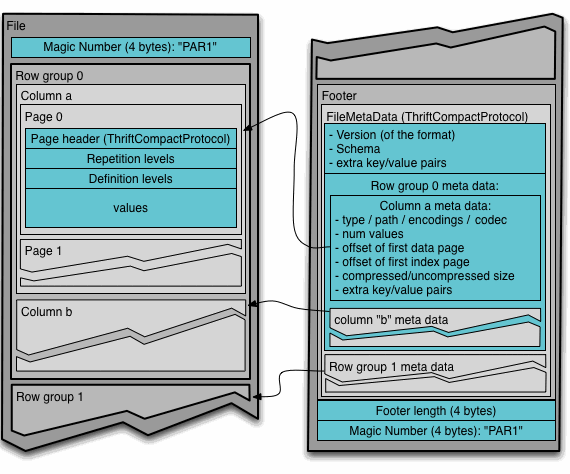
\includegraphics[width=10.5cm]{./assets/img/parquet.png}
	\caption{Parquet file structure}
	\label{fig:parque_file_structuret}
	\vspace{0.5cm}
\end{figure}

In addition to data types, as described in \figurename~\ref{fig:parque_file_structuret}, Parquet stores metadata at three levels: file metadata, column chunk metadata and page header metadata. The file metadata contains: \\

\begin{itemize}
	\begin{minipage}{0.92\textwidth}
		\item The version of the Parquet format  \\
	\end{minipage} \\
	\begin{minipage}{0.92\textwidth}
		\item The data schema \\
	\end{minipage} \\
	\begin{minipage}{0.92\textwidth}
		\item The column metadata, which include its type, the number of values, its location and the encoding schema \\
	\end{minipage} \\
	\begin{minipage}{0.92\textwidth}
		\item Additional key-value pairs \\
	\end{minipage}
\end{itemize}

The file metadata are written after the data to allow single pass writing. Then, to determine which column chunks should be read, the readers first check the file metadata to find them. The columns chunks should then be read sequentially.

The row group column chunk metadata are contained in the footer as well and include statistics for their data pages such as min/max, and can be used to skip pages when scanning data in ordered and unordered columns. In the previous versions of the format this was not possible, since statistics were stored in the column and data page headers. Thus, when reading pages, a reader had to process the page header to determine whether the page could be skipped based on the statistics or not.

It is important to emphasise that the format is explicitly designed to separate the metadata from the data. This allows splitting columns into multiple files, as well as having a single metadata file reference multiple parquet files. Indeed, Parquet allows to split the files in any desirable size. This may be particularly advantageous when working with gigabytes or terabytes of data and in parallel environments.

As already stated, Parquet has been developed taking inspiration from Dremel. Then Parquet uses its encoding with definition and repetition levels. For data pages, three pieces of information are encoded back to back, after the page header: the definition levels data, the repetition levels data and the encoded values. However, if the column is non-nested and required, the data in the page are just the encoded values. The size of a data page is specified in its header and it includes all its 3 parts combined, with the information about compression and encoding. Data pages share also a common column header to allow readers to skip over pages they are not interested in.

\subsection{Apache Arrow}

\label{subsection:arrow}

\textit{Apache Arrow} is a software development platform for building high performance applications that process and transport large data sets. It aims to improve the performance of analytical algorithms and the efficiency of transferring data from one system or programming language to another\cite{arrow_overview}.

In other words, Arrow is a cross-language development platform for in-memory analytics\cite{arrow_homepage}. Indeed, its in-memory binary columnar format is a standardized, language-agnostic specification for representing structured, table-like data sets, in-memory. It is important to emphasise that Arrow does not provide any compression and encoding mechanisms. Arrow used alone is just a way to represent data in-memory. It is therefore not surprising that a data set represented in Arrow format is larger in size than a data set represented in \texttt{.csv} or any other textual format.

As in ORC, this format has a rich data type system that includes nested and user-defined data types, designed to support the needs of analytic database systems, data frame libraries, and more\cite{arrow_overview}. The key aspects of Arrow are the following: \\

\begin{itemize}
	\begin{minipage}{0.92\textwidth}
		\item \begin{multicols}{2}
			Using a columnar storage format allows execution engines such as Apache Spark to maximize their efficiency when scanning and iterating large chunks of data. To achieve this goal, the contiguous columnar layout supports vectorization using the latest SIMD (Single Instruction, Multiple Data) operations included in modern processors
			\columnbreak
			\begin{center}
				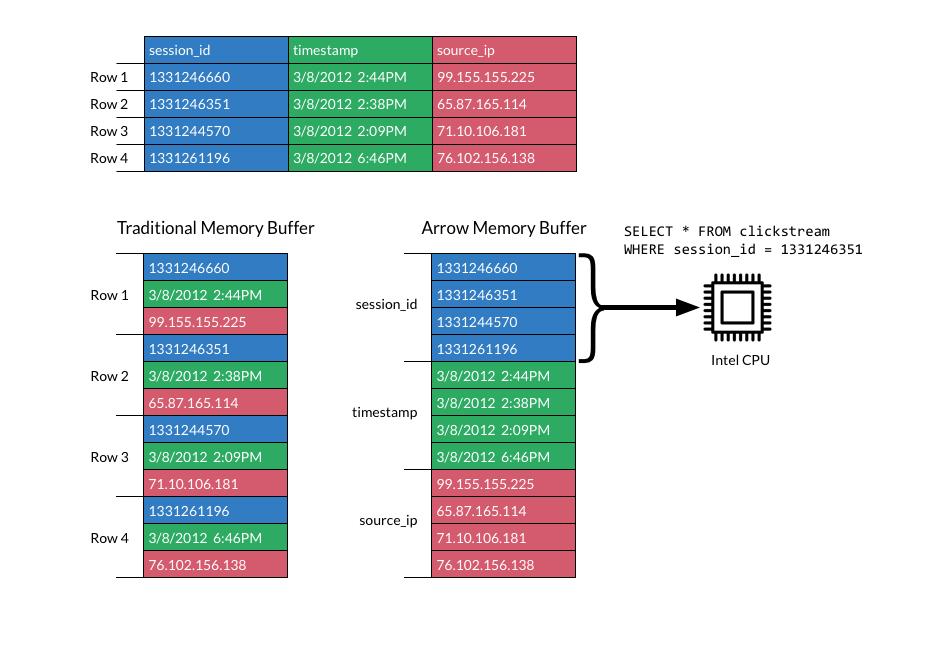
\includegraphics[height=5.5cm,width=7cm]{./assets/img/arrow/arrow_columnar_storage.png}
			\end{center}
		\end{multicols}
	\end{minipage} \\
	\begin{minipage}{0.92\textwidth}
		\item \begin{multicols}{2}
			Due to the lack of a standard columnar data format, every database and language has to implement its own internal data format. This implies a lot of waste when moving data from one system to another and causes costly serialization and de-serialization processes, as shown in the first image on the right. In addition, common algorithms must often be rewritten for each data format.
			\columnbreak
			\begin{center}
				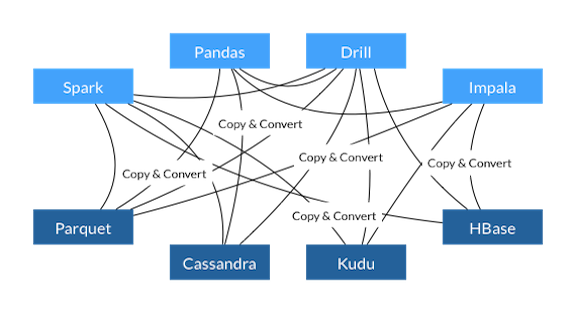
\includegraphics[height=5cm,width=6.5cm]{./assets/img/arrow/without_arrow.png}
			\end{center}
		\end{multicols}
		\begin{multicols}{2}
			As remarked in the second image on the right, Arrow's in-memory columnar data format represent then an out-of-the-box solution to these problems. Indeed, systems using or supporting Arrow can transfer data between them at little-to-no cost and do not need to implement custom connectors for every other system. On top of these savings, a standardized memory format facilitates re-use of libraries of algorithms, even across languages
			\columnbreak
			\begin{center}
				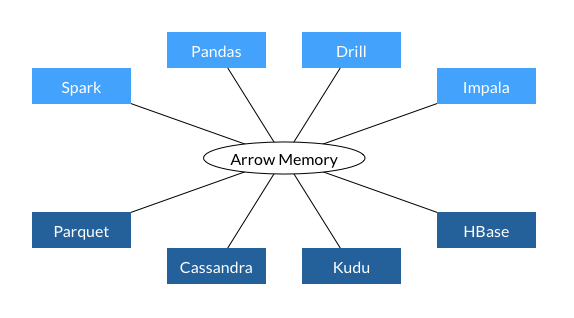
\includegraphics[height=5cm,width=6.5cm]{./assets/img/arrow/with_arrow.png}
			\end{center}
		\end{multicols}
	\end{minipage} \\
	\begin{minipage}{0.92\textwidth}
		\item As Arrow can be used in very different systems and projects, its native libraries are available for the following programming languages: C\texttt{++}, C\#, Go, Java, JavaScript, Julia and Rust. However, Arrow's libraries are also available for C, MATLAB, Python, R and Ruby. These libraries are built on top of the C\texttt{++} library.
		The project also contains utilities for reading and writing it to many common storage formats, among which Parquet.
		Finally, the Arrow libraries contain many software components that solve system problems related to retrieving and sending data to and from remote storage systems and moving data in Arrow format over network interfaces. Indeed, some of these components can be used even in scenarios where the columnar format is not used at all\cite{arrow_overview}
	\end{minipage} \\
\end{itemize}

In order to store data, Arrow uses arrays, i.e. a sequence of values with known length all having the same type. Arrays are defined by a few pieces of metadata and data. They contain: \\

\begin{itemize}
	\begin{minipage}{0.92\textwidth}
		\item A logical data type \\
	\end{minipage} \\
	\begin{minipage}{0.92\textwidth}
		\item A sequence of buffers, which are sequential virtual address spaces with a given length \\
	\end{minipage} \\
	\begin{minipage}{0.92\textwidth}
		\item A length as either 64-bit or 32-bit signed integer \\
	\end{minipage} \\
	\begin{minipage}{0.92\textwidth}
		\item A \texttt{null} count as a 64-bit signed integer \\
	\end{minipage} \\
	\begin{minipage}{0.92\textwidth}
		\item An optional dictionary for dictionary-encoded arrays \\
	\end{minipage}
\end{itemize}

Nested types, which are data types whose full structure depends on one or more other child types such as lists, use nested arrays. These nested arrays additionally have a sequence of one or more sets of these items, called child arrays.

Each logical data type has a well-defined physical layout. Here are the different physical layouts defined by Arrow\cite{arrow_format}: \\

\begin{itemize}
	\begin{minipage}{0.92\textwidth}
		\item Primitive, a sequence of values that all have the same width of bytes or bits \\
	\end{minipage} \\
	\begin{minipage}{0.92\textwidth}
		\item Variable-size binary, a sequence of values each with a variable byte length. This layout supports 32-bit and 64-bit encoding \\
	\end{minipage} \\
	\begin{minipage}{0.92\textwidth}
		\item Fixed-size list, a nested layout where each value has the same number of elements taken from a child data type. \\
	\end{minipage} \\
	\begin{minipage}{0.92\textwidth}
		\item Variable-size list, a nested layout where each value is a sequence of values each with a variable byte length of values taken from a child data type \\
	\end{minipage} \\
	\begin{minipage}{0.92\textwidth}
		\item Struct, a nested layout consisting of a collection of named child fields each having the same length, possibly having different types \\
	\end{minipage} \\
	\begin{minipage}{0.92\textwidth}
		\item Sparse and dense union, nested layouts representing a sequence of values possibly having different types \\
	\end{minipage} \\
	\begin{minipage}{0.92\textwidth}
		\item Null, a sequence of all null values \\
	\end{minipage}
\end{itemize}

Each logical type uses one of the physical layouts described above. However, nested logical types may have different physical layouts depending on the particular realization of the type. As stated in the official Arrow documentation, the list of supported logical types can be found at the following link: \href{https://github.com/apache/arrow/blob/master/format/Schema.fbs}{https://github.com/apache/arrow/blob/master/format/Schema.fbs}

However the Arrow columnar memory layout only applies to data and not to metadata. Metadata serialization is obtained using the Google’s \textit{Flatbuffers}\cite{flatbuffers}.

\subsubsection{Comparison to CarbonData, Parquet and ORC}

While Parquet and ORC are examples of on-disk columnar data formats, Arrow is a runtime in-memory format. The former file formats almost always have to be deserialized into some in-memory data structure for processing. The goal of Arrow is to be that in-memory data structure and to be a complement to these formats\cite{arrow_faq}. On-disk columnar formats are designed to maximize space efficiency, using advanced compression and encoding techniques. Then they are the best choice when the goal is to minimize disk usage while storing tons of data. However, this efficiency comes at the cost of relatively expensive reading into memory. Conversely, Arrow is an in-memory format meant for direct and efficient use for computational purposes. Indeed, default Arrow data are not compressed.

Currently, Arrow and Parquet complement each other since both projects includes libraries that allow reading and writing data in the other format.

\section{Compression algorithms}

\label{section:compression_algorithms}

All the formats described use \textit{Snappy}\cite{google_snappy} as default compression algorithm, but since CarbonData, ORC and Parquet compress the data to provide an highly efficient way to store them, the choice of the compression algorithm is a key aspect that has to be analyzed, as it affects both storage and query efficiency. Indeed, compression helps to reduce the resources required to store and transmit data.

Each columnar storage format supports its own compression algorithms. In details: \\

\begin{itemize}
	\begin{minipage}{0.92\textwidth}
		\item
		CarbonData supports snappy, zstd and gzip \\
	\end{minipage} \\
	\begin{minipage}{0.92\textwidth}
		\item
		ORC supports snappy, lzo and zlib \\
	\end{minipage} \\
	\begin{minipage}{0.92\textwidth}
		\item
		Parquet supports snappy, lz4, brotli\cite{google_brotli}, gzip, zstd, lzo \\
	\end{minipage}
\end{itemize}

All the algorithms supported are therefore, to a greater or lesser extent, dictionary-based compression algorithms. In other words, all supported algorithms are lossless data compression algorithms that operate by searching for matches between the text to be compressed and a set of strings contained in a data structure called ``dictionary''.

\textit{Snappy}\cite{google_snappy} is a fast open-source data compression and decompression library implemented in C\texttt{++} and developed by Google, based on LZ77. Its encoding is byte-oriented and does not use entropy encoder. It is not only fast, but also stable and robust. For these reasons, Snappy is widely used inside Google solutions.

\textit{ZStandard}\cite{facebook_zstd}, better known as zstd, is a fast open-source compression algorithm implemented in C and developed by Facebook. ZStandard combines the ideas of LZ77 with a large search window and entropy encoding. Despite its youth, it is already used in several systems.

\textit{Zlib}\cite{zlib} is a software library implemented in C used for data compression, written by Jean-loup Gailly and Mark Adler. It provides the \texttt{DEFLATE} algorithm, a replacement for LZW, which is a combination of LZ77 and Huffman encoding. Its compression and decompression procedures are used by zip, gzip, png, et cetera.

\textit{GNU Gzip}\cite{gnu_gzip} is a popular compression and decompression wrapper for zlib written for the GNU project\cite{gnu_project} by Jean-loup Gailly and Mark Adler. It is free and it was designed to replace the compress program used in early Unix systems.

\textit{Lempel–Ziv–Oberhumer}\cite{lzo} is an open-source compression algorithm implemented in C by Markus F.X.J. Oberhumer, focused on decompression speed. LZO compresses a block of data using a LZ77 sliding dictionary. It is also based on the \texttt{DEFLATE} algorithm. It is used in various systems.

\textit{Lz4}\cite{lz4} is a fast data compression algorithm implemented in C by Yann Collet, with the aim to provide a good trade-off between speed and compression ratio. Unlike other compression algorithms, it uses only a dictionary-matching stage based on LZ77 avoiding to combine it with an entropy encoding.

\textit{Brotli}\cite{google_brotli} is a compression algorithm implemented in C by Google. It uses a combination of a modern variant of the LZ77 algorithm, Huffman coding and 2nd order context modeling. It works best for text compression and it is widely used in web contexts.

Despite the formats supports these algorithms, some of of them still lack the implementation in the Hadoop environment and are not easy-to-use.

In order to detect those algorithms that work best, the \textit{Squash Compression Benchmark}\cite{squash_compression_benchmark} it has been used. This tool is part of the \textit{Squash} library, that is an abstraction layer for compression algorithms. Indeed, Squash provides a single API to access many compression libraries, allowing applications a great deal of flexibility in choosing compression algorithms. The Squash Compression Benchmark currently consists of 28 data sets and is currently running on 9 different machines.

The choice of the data set \textit{urls.10K}\cite{urls_dataset} has been rather obvious as RDF triples are mostly composed of URIs, whereas the running machine has been assigned randomly.

The following factors were taken into account when evaluating the different algorithms: \\

\begin{itemize}
	\begin{minipage}{0.92\textwidth}
		\item
		$\text{ratio} = \frac{\text{uncompressed size}}{\text{compressed size}}$ \\
	\end{minipage} \\
	\begin{minipage}{0.92\textwidth}
		\item
		$\text{compression speed} = \frac{\text{uncompressed size}}{\text{compression time}}$ \\
	\end{minipage} \\
	\begin{minipage}{0.92\textwidth}
		\item
		$\text{decompression speed} = \frac{\text{uncompressed size}}{\text{decompression time}}$ \\
	\end{minipage}
\end{itemize}

Figures \ref{fig:ratio_compress}, \ref{fig:ratio_decompress}, \ref{fig:compress_decompress} show the results obtained using the \textit{satellite-a205} machine, equipped with an Intel Celeron 540 running at 1.86 GHz with 1 GB RAM\footnote{The plots show for each compression algorithm either different levels of application or different variants of the same core algorithms. The level indicates how aggressively the algorithms work to compress a file. The conclusions drawn are therefore to be understood in terms of average performance}.

\begin{figure}
	\centering
	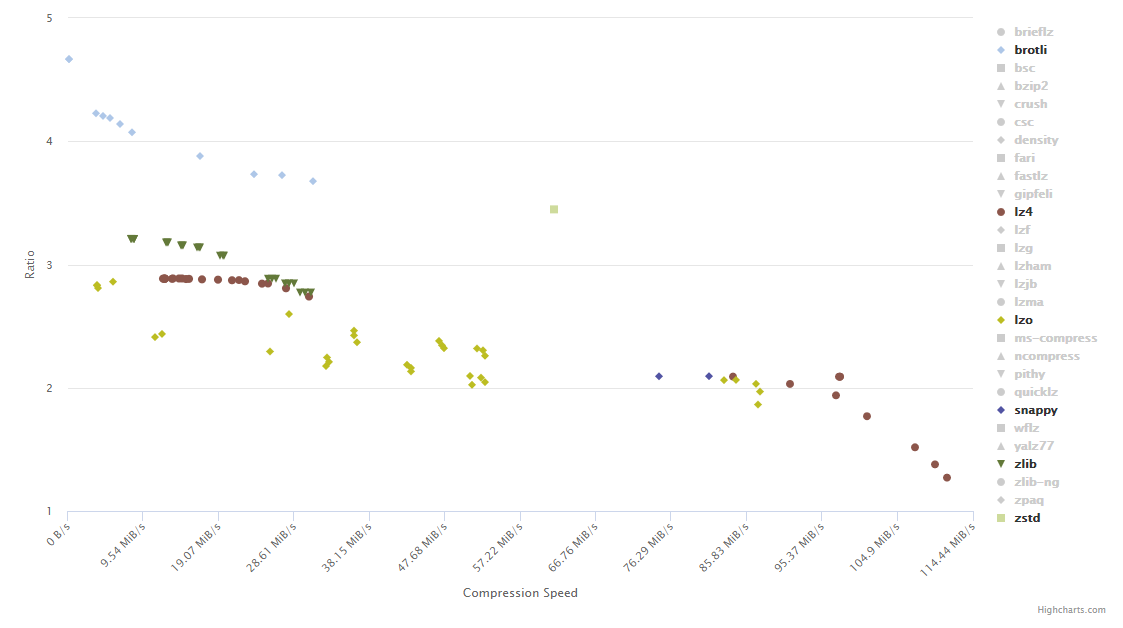
\includegraphics[width=15cm]{./assets/img/squash/ratio_compress.png}
	\caption{Compression ratio vs. compression speed}
	\label{fig:ratio_compress}
	\vspace{0.5cm}
\end{figure}
\begin{figure}
	\centering
	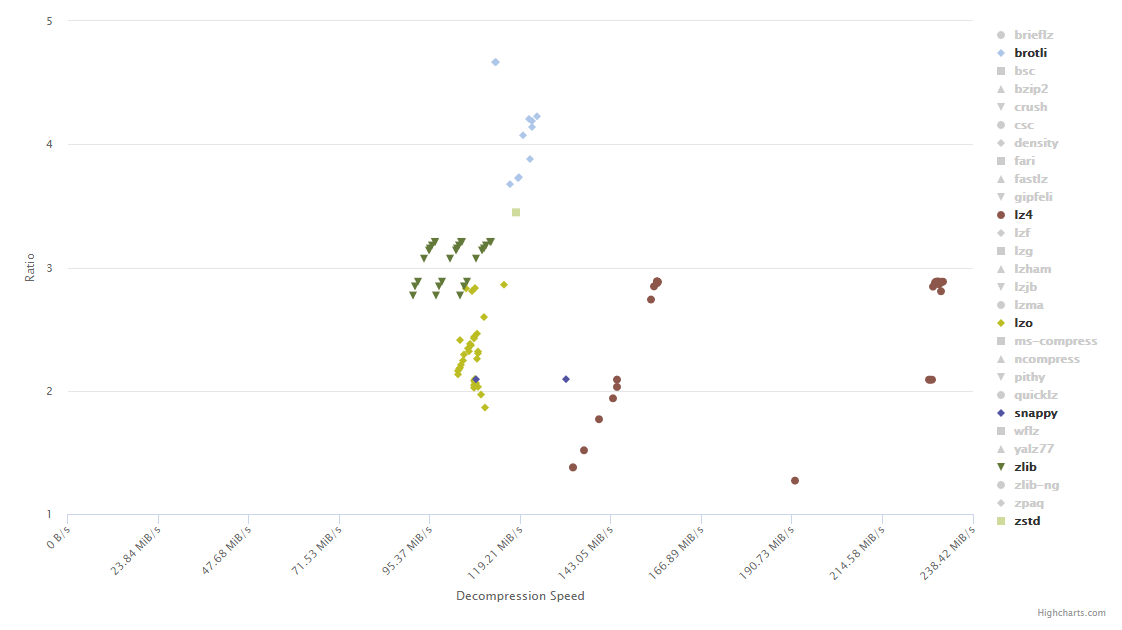
\includegraphics[width=15cm]{./assets/img/squash/ratio_decompress.png}
	\caption{Compression ratio vs. decompression speed}
	\label{fig:ratio_decompress}
	\vspace{0.5cm}
\end{figure}
\begin{figure}
	\centering
	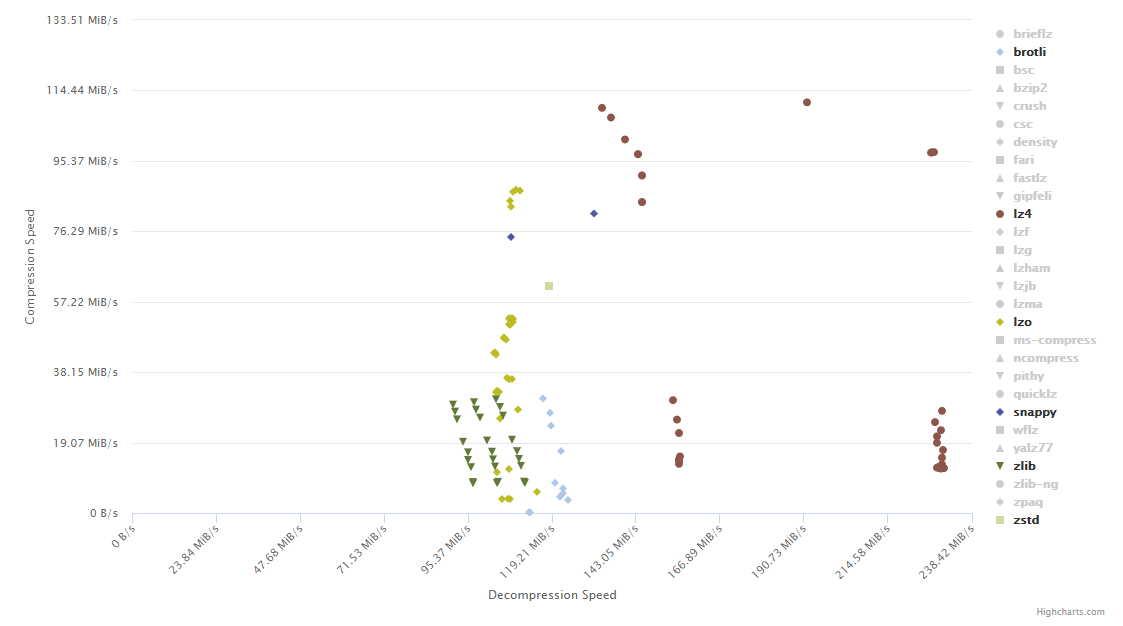
\includegraphics[width=15cm]{./assets/img/squash/compress_decompress.png}
	\caption{Compression speed vs. decompression speed}
	\label{fig:compress_decompress}
	\vspace{0.5cm}
\end{figure}

Obviously, which algorithm works best depends on the trade-off between space and speed to be achieved, but it is possible to identify some algorithms that work better than others and draw the following conclusions: \\

\begin{itemize}
	\begin{minipage}{0.92\textwidth}
		\item Surely, lz4 seems to perform better than snappy in all three comparison metrics, and it is the best choice when the key aspect is the compression/decompression speed. Moreover it is preferable to lzo as well, given the minimal disk footprint advantage achieved with it \\
	\end{minipage} \\
	\begin{minipage}{0.92\textwidth}
		\item Overall, snappy and lzo seems to perform really similar \\
	\end{minipage} \\
	\begin{minipage}{0.92\textwidth}
		\item In terms of disk footprint, brotli performs best and it is preferable to zlib and lzo \\
	\end{minipage} \\
	\begin{minipage}{0.92\textwidth}
		\item Overall, zstd might be good compromise among the different evaluation metrics \\
	\end{minipage} \\
	\begin{minipage}{0.92\textwidth}
		\item Overall, zlib seems to perform poorly \\
	\end{minipage}
\end{itemize}

Nonetheless, brotli and zstd still lack the implementation in the Hadoop environment and are not easy-to-use. Hence, Parquet has been evaluated using snappy and lz4, ORC with snappy and lzo, while CarbonData just with snappy.

\chapter{Literature Review}

\label{chapter:literature_review}

The objective of this concise chapter is to describe some of the most famous RDF stores based on the triples table which are currently used, in order to make the reader aware of current alternatives. However, unlike the RDF storage analyzed in this work, most of them use other tables in order to speed up the data retrieval mechanism and perform joins and have a heavier indexing mechanism. An important source of information for this chapter is the survey conducted by Ali et al.\cite{rdf_store_survey}.

\textit{3store}\cite{3store} is a MySQL based triple store and it uses 3 additional tables. Indeed, beyond the triples table there are the models, the resource and the literal table. Those tables have two-columns that encode data models, resources and literals respectively. As in this work, the SPARQL queries are translated to SQL before being executed.

\textit{RDF-3X}\cite{rdf3x} stores its triples table using compressed indexes, which are based on clustered B\textsuperscript{+}trees. RDF-3X does not rely on a classical RDBMS, but rather depends on its own storage system, specifically designed to accommodate RDF data. In addition to the classic triple table, it stores all its possible permutations. Thus, by identifying the subject column with S, the predicate column with P and the object column with O, RDF-3X stores the tables SPO, SOP, OSP, OPS, PSO and POS. It uses these table to perform fast indexing but on the other hand the memory footprint is not insignificant. To reduce it, RDF-3X uses a dictionary-based encoding.

\textit{LuposDate}\cite{luposdate} is a semantic web DBMS that stores the table of triples by annotating them with a rank. These ranks are constructed from the six permutations of the triple and are used for fast sorting when applying sort-merge joins. Moreover, it also uses 7 hash indexes: S, P, O, SP, SO, PO, SPO.

\textit{Apache Jena TDB}\cite{jena_tdb} is a component of the Apache Jena\cite{jena} framework for RDF storage and query. It can be used as a high performance RDF store on a single machine. To store the data, it uses custom B\textsuperscript{+}trees while the SPARQL engine is implemented in the custom Jena ARQ\cite{jena_arq} query processor. Jena TDB, that is now the recommended RDF store for Jena, was preceded by Jena SDB\cite{jena_sdb}, another relation-based storage that is no longer supported. It stores the data in a three or four columns table.

\textit{Virtuoso}\cite{virtuoso} is a system produced by OpenLink which has encountered many changes in the previous years. It was originally developed as an RDBMS, but now is probably one of the most famous RDF storage. It was implemented with a row-storage approach, but now presents a hybrid approach by supporting column-store features. Virtuoso stores RDF data as a quad table instead of the classic three-column table. The fourth column describes the triple membership graph. Identifying the fourth column with G, the quad table includes five indexes by default in the most recent version: PSOG, POGS, SP, OP and GS. All elements except the objects are dictionary encoded. The query engine needs to translate SPARQL queries into SQL before executing them in the underlying database.

\textit{RDFJoin}\cite{rdfjoin} is a persistent column-store database. It stores the triples using three types of tables: dictionary, triples and join tables. The two dictionary tables are used to encode and decode the elements. The triples table are three. Each of them uses two columns as primary key, while the remaining column is encoded as a bit vector. The join tables store the results of S-S, O-O and S-O column joins. RDFJoin relies on either \textit{MonetDB} or \textit{LucidDB}. It supports SPARQL but not inference.

\textit{RDFKB}\cite{rdfkb} is a RDBMS implemented as a column-store that uses the RDFJoin technology. The key feature of this solution is the fact that for each triple RDFKB infers all possible additional RDF triples, stores and makes them accessible to queries. However, this implies redundant information, then more storage space and memory consumption.

\textit{RDFox}\cite{rdfox} is a highly scalable in-memory RDF store and a semantic reasoning engine as well. The storage is implemented using linked lists that beyond the subject, predicate and object, store three pointers to the next triple with the same subject, predicate and object respectively. The indexes are built using hash tables. RDFox's key feature is its support to shared memory parallel reasoning and to SPARQL 1.1.

\textit{TripleID-Q}\cite{tripleidq} is a RDF store that uses a triples representation called Triple-ID. This representation is based on dictionary encoding. It is smaller than the original representation 3-4 times and allows query processing on GPUs. Indeed, rather than indexing the triples, small chunks of the table can be loaded on GPU. The key features of TripleID-Q are then: the compact representation suitable for GPU, the simple representation conversion method which optimizes the pre-processing and the parallel algorithms which use GPUs to seek specific data.

\chapter{Research methodology, experiments and results}

The objective of this work is to evaluate the suitability of some columnar storage formats, namely CarbonData, ORC, Parquet and Arrow, for the RDF data model, in terms of disk footprint and query time, when dealing with Big Data in a real cloud context. Thus, this experimentation conducted using Apache Spark first in a local environment and then in a cluster of machines using AWS\cite{aws} as cloud provider, should allow the identification of the most suitable format in the context of Big Data and cloud computing.

The ease of use of each format in the different environments used will also be discussed and evaluated, since in some cases, for some formats, it was not possible either to store the data using the current format or to execute the queries due to the lack of support and documentation, or to the non-compatibility with the environment.

\section{Research methodology and experiments}

\label{section:research_methodology}

While the method used to obtain disk footprint information changes depending on the environment and will be discussed later, the method of collecting query time information was always the same. Indeed, once the storages were queried using the Spark SQL framework, query time information was collected using the SQL tab of Spark UI. This tab displays information, such as the duration, jobs, and physical and logical plans for queries. Accurately, each query has been executed just one time to avoid the exchange re-use of Spark. Indeed, when Spark runs shuffling (i.e. aggregation, join, et cetera), it stores a copy of the shuffle data on local worker nodes for potential re-use. This, obviously, allows Spark to re-use cached result for potentially faster query performance.

In order to evaluate the formats and their performances a famous benchmark RDF data set, i.e. the Lehigh University Benchmark dataset, from now on \textit{LUBM} has been used. But before being usable, it needed pre-processing as the data set triples were distributed over thousand files. Therefore, the first step was to merge the triples into a single unique file using a simple \textit{Python} script. Later, as the LUBM dataset was obtained in RDF/XML, it has been converted to N-Triples using the tool \textit{rdf2rdf}\cite{rdf2rdf} to avoid further pre-processing, since its data representation is really similar to the one obtained using columnar storage, i.e. a 3 column-table.

Then, the data set has been tested using simple SPARQL queries, i.e queries without \texttt{FILTER}, \texttt{JOIN}, \texttt{OPTIONAL} et cetera. In order to execute them using the Spark SQL framework, all the queries have been translated to the classic SQL syntax. To achieve this, the \textit{Basic Graph Pattern}, from now on BGP, of all queries has been retrieved using the Apache Jena ARQ query engine\cite{jena_arq}. BGPs are sets of triple patterns. Then, the SPARQL graph pattern matching mechanism is defined in terms of combining the results from matching basic graph patterns. Once BGPs have been obtained, a simplification of the BGPtoSQL algorithm has been implemented to translate to SQL the easy-to-translate queries. Here it follows the basic procedure: \\

\begin{enumerate}
	\begin{minipage}{0.92\textwidth}
		\item Assign a unique table alias to every triple pattern \\
	\end{minipage} \\
	\begin{minipage}{0.92\textwidth}
		\item Construct the \texttt{FROM} clause to contain all table aliases \\
	\end{minipage} \\
	\begin{minipage}{0.92\textwidth}
		\item Construct the \texttt{SELECT} clause to contain every relation attribute that corresponds to a distinct variable \\
	\end{minipage} \\
	\begin{minipage}{0.92\textwidth}
		\item Construct the \texttt{WHERE} clause to restrict attribute values to the corrisponding URIs and literals \\
	\end{minipage} \\
	\begin{minipage}{0.92\textwidth}
		\item Finalize the \texttt{WHERE} clause to ensure that the same variables used in different triple patterns must have the same value \\
	\end{minipage}
\end{enumerate}

\subsection{LUBM}

The \textit{Lehigh University Benchmark}, i.e. LUBM, has been developed to facilitate the performance evaluation of Semantic Web repositories in a standard and systematic way, with respect to extensional queries over a large dataset that commits to a single ontology\cite{lubm_dataset_paper}. It consists of 2 softwares, a university domain ontology, a set of test queries and several performance metrics.

\subsubsection{Pre-processing}

As already claimed, the LUBM does not contain a data set, but a software to generate it over the \textit{Univ-Bench}\cite{univ_ontology} ontology in the unit of a university. The data generation process is repeatable and customizable, by specifying seed for random number generation, the number of universities and the starting index of the universities.
Using this software, the following data sets have been generated\footnote{It was originally planned to generate also \textit{lubm10000}, but due to the high computational complexity, it was decided to evaluate data sets under 30 GB}: \textit{lubm1}, \textit{lubm10}, \textit{lubm100} and \textit{lubm1000}. The numbers associated with LUBM, refers to the number of universities setted during the data set generation.

However, the software generates thousands of files. Then, as mentioned above, these files have been merged using a simple Python script and then translated from RDF/XML to N-Triples using the \textit{rdf2rdf} tool.

\subsubsection{Queries}

\label{subsubsection:lubm_queries}

The benchmark currently provides 14 test queries written in SPARQL 1.0 syntax. Here it follows the list of the simple queries\footnote{In order not to be redundant, the following common prefixes have been omitted:
	\vspace{0.1cm} \\
	\hspace*{0.8cm}\lstinline[language=sql]{PREFIX rdf: <http://www.w3.org/1999/02/22-rdf-syntax-ns#>} \\
	\hspace*{0.8cm}\lstinline[language=sql]{PREFIX ub: <http://www.lehigh.edu/~zhp2/2004/0401/univ-bench.owl#>} \\
}:\\

\begin{enumerate}
	\begin{minipage}{0.92\textwidth}
		\item \label{query:lumb_sparql_1}
		\lstset{language=sql}
		\begin{lstlisting}
SELECT ?X
WHERE {
    ?X rdf:type ub:GraduateStudent .
    ?X ub:takesCourse <http://www.Department0.University0.edu/GraduateCourse0>
}
                        \end{lstlisting}
	\end{minipage} \\
	\begin{minipage}{0.92\textwidth}
		\item \label{query:lumb_sparql_2}
		\lstset{language=sql}
		\begin{lstlisting}
SELECT ?X ?Y ?Z
WHERE {
    ?X rdf:type ub:GraduateStudent .
    ?Y rdf:type ub:University .
    ?Z rdf:type ub:Department .
    ?X ub:memberOf ?Z .
    ?Z ub:subOrganizationOf ?Y .
    ?X ub:undergraduateDegreeFrom ?Y
}
                        \end{lstlisting}
	\end{minipage} \\
	\begin{minipage}{0.92\textwidth}
		\item \label{query:lumb_sparql_3}
		\lstset{language=sql}
		\begin{lstlisting}
SELECT ?X
WHERE {
    ?X rdf:type ub:Publication .
    ?X ub:publicationAuthor <http://www.Department0.University0.edu/AssistantProfessor0>
}
                        \end{lstlisting}
	\end{minipage} \\
	\begin{minipage}{0.92\textwidth}
		\item \label{query:lumb_sparql_4}
		\lstset{language=sql}
		\begin{lstlisting}
SELECT ?X ?Y1 ?Y2 ?Y3
WHERE {
    ?X rdf:type ub:Professor .
    ?X ub:worksFor <http://www.Department0.University0.edu> .
    ?X ub:name ?Y1 .
    ?X ub:emailAddress ?Y2 .
    ?X ub:telephone ?Y3
}
                        \end{lstlisting}
	\end{minipage} \\
	\begin{minipage}{0.92\textwidth}
		\item \label{query:lumb_sparql_5}
		\lstset{language=sql}
		\begin{lstlisting}
SELECT ?X
WHERE {
    ?X rdf:type ub:Person .
    ?X ub:memberOf <http://www.Department0.University0.edu>
}
                        \end{lstlisting}
	\end{minipage} \\
	\begin{minipage}{0.92\textwidth}
		\item \label{query:lumb_sparql_6}
		\lstset{language=sql}
		\begin{lstlisting}
SELECT ?X
WHERE {
    ?X rdf:type ub:Student
}
                        \end{lstlisting}
	\end{minipage} \\
	\begin{minipage}{0.92\textwidth}
		\item \label{query:lumb_sparql_7}
		\lstset{language=sql}
		\begin{lstlisting}
SELECT ?X ?Y
WHERE {
    ?X rdf:type ub:Student .
    ?Y rdf:type ub:Course .
    ?X ub:takesCourse ?Y .
    <http://www.Department0.University0.edu/AssociateProfessor0> ub:teacherOf ?Y
}
                        \end{lstlisting}
	\end{minipage} \\
	\begin{minipage}{0.92\textwidth}
		\item \label{query:lumb_sparql_8}
		\lstset{language=sql}
		\begin{lstlisting}
SELECT ?X ?Y ?Z
WHERE {
    ?X rdf:type ub:Student .
    ?Y rdf:type ub:Department .
    ?X ub:memberOf ?Y .
    ?Y ub:subOrganizationOf <http://www.University0.edu> .
    ?X ub:emailAddress ?Z
}
                        \end{lstlisting}
	\end{minipage} \\
	\begin{minipage}{0.92\textwidth}
		\item \label{query:lumb_sparql_9}
		\lstset{language=sql}
		\begin{lstlisting}
SELECT ?X ?Y ?Z
WHERE {
    ?X rdf:type ub:Student .
    ?Y rdf:type ub:Faculty .
    ?Z rdf:type ub:Course .
    ?X ub:advisor ?Y .
    ?Y ub:teacherOf ?Z .
    ?X ub:takesCourse ?Z
}
                        \end{lstlisting}
	\end{minipage} \\
	\begin{minipage}{0.92\textwidth}
		\item \label{query:lumb_sparql_10}
		\lstset{language=sql}
		\begin{lstlisting}
SELECT ?X
WHERE {
    ?X rdf:type ub:Student .
    ?X ub:takesCourse <http://www.Department0.University0.edu/GraduateCourse0>
}
                        \end{lstlisting}
	\end{minipage} \\
	\begin{minipage}{0.92\textwidth}
		\item \label{query:lumb_sparql_11}
		\lstset{language=sql}
		\begin{lstlisting}
SELECT ?X
WHERE {
    ?X rdf:type ub:ResearchGroup .
    ?X ub:subOrganizationOf <http://www.University0.edu>
}
                        \end{lstlisting}
	\end{minipage} \\
	\begin{minipage}{0.92\textwidth}
		\item \label{query:lumb_sparql_12}
		\lstset{language=sql}
		\begin{lstlisting}
SELECT ?X ?Y
WHERE {
    ?X rdf:type ub:Chair .
    ?Y rdf:type ub:Department .
    ?X ub:worksFor ?Y .
    ?Y ub:subOrganizationOf <http://www.University0.edu>
}
                        \end{lstlisting}
	\end{minipage} \\
	\begin{minipage}{0.92\textwidth}
		\item \label{query:lumb_sparql_13}
		\lstset{language=sql}
		\begin{lstlisting}
SELECT ?X
WHERE {
    ?X rdf:type ub:Person .
    <http://www.University0.edu> ub:hasAlumnus ?X
}
                        \end{lstlisting}
	\end{minipage} \\
	\begin{minipage}{0.92\textwidth}
		\item \label{query:lumb_sparql_14}
		\lstset{language=sql}
		\begin{lstlisting}
SELECT ?X
WHERE {
    ?X rdf:type ub:UndergraduateStudent
}
                        \end{lstlisting}
	\end{minipage} \\
\end{enumerate}

As already mentioned, these queries had to be translated into SQL before being executed. Below are the translated queries obtained by running the BGPtoSQL algorithm: \\

\begin{enumerate}
	\begin{minipage}{0.92\textwidth}
		\item \label{query:lumb_sql_1}
		\lstset{language=sql}
		\begin{lstlisting}
SELECT t1.subject AS X
FROM triples AS t1, triples AS t2
WHERE t1.object = ``<http://swat.cse.lehigh.edu/onto/univ-bench.owl#GraduateStudent>''
AND t1.predicate = ``<http://www.w3.org/1999/02/22-rdf-syntax-ns#type>''
AND t2.predicate = ``<http://swat.cse.lehigh.edu/onto/univ-bench.owl#takesCourse>''
AND t2.object = ``<http://www.Department0.University0.edu/GraduateCourse0>''
AND t1.subject = t2.subject
                        \end{lstlisting}
	\end{minipage} \\
	\begin{minipage}{0.92\textwidth}
		\item \label{query:lumb_sql_2}
		\lstset{language=sql}
		\begin{lstlisting}
SELECT t1.subject AS X, t2.subject AS Y, t3.subject AS Z
FROM triples AS t1, triples AS t2, triples AS t3, triples AS t4, triples AS t5, triples AS t6
WHERE t1.object = ``<http://swat.cse.lehigh.edu/onto/univ-bench.owl#GraduateStudent>''
AND t1.predicate = ``<http://www.w3.org/1999/02/22-rdf-syntax-ns#type>''
AND t2.object = ``<http://swat.cse.lehigh.edu/onto/univ-bench.owl#University>''
AND t2.predicate = ``<http://www.w3.org/1999/02/22-rdf-syntax-ns#type>''
AND t3.object = ``<http://swat.cse.lehigh.edu/onto/univ-bench.owl#Department>''
AND t3.predicate = ``<http://www.w3.org/1999/02/22-rdf-syntax-ns#type>''
AND t4.predicate = ``<http://swat.cse.lehigh.edu/onto/univ-bench.owl#memberOf>''
AND t5.predicate = ``<http://swat.cse.lehigh.edu/onto/univ-bench.owl#subOrganizationOf>''
AND t6.predicate = ``<http://swat.cse.lehigh.edu/onto/univ-bench.owl#undergraduateDegreeFrom>''
AND t1.subject = t4.subject
AND t4.subject = t6.subject
AND t2.subject = t5.object
AND t5.object = t6.object
AND t3.subject = t4.object
AND t4.object = t5.subject
                        \end{lstlisting}
	\end{minipage} \\
	\begin{minipage}{0.92\textwidth}
		\item \label{query:lumb_sql_3}
		\lstset{language=sql}
		\begin{lstlisting}
SELECT t1.subject AS X
FROM triples AS t1, triples AS t2
WHERE t1.object = ``<http://swat.cse.lehigh.edu/onto/univ-bench.owl#Publication>''
AND t1.predicate = ``<http://www.w3.org/1999/02/22-rdf-syntax-ns#type>''
AND t2.predicate = ``<http://swat.cse.lehigh.edu/onto/univ-bench.owl#publicationAuthor>''
AND t2.object = ``<http://www.Department0.University0.edu/AssistantProfessor0>''
AND t1.subject = t2.subject
                        \end{lstlisting}
	\end{minipage} \\
	\begin{minipage}{0.92\textwidth}
		\item \label{query:lumb_sql_4}
		\lstset{language=sql}
		\begin{lstlisting}
SELECT t1.subject AS X, t3.object AS Y1, t4.object AS Y2, t5.object AS Y3
FROM triples AS t1, triples AS t2, triples AS t3, triples AS t4, triples AS t5
WHERE t1.object = ``<http://swat.cse.lehigh.edu/onto/univ-bench.owl#Professor>''
AND t1.predicate = ``<http://www.w3.org/1999/02/22-rdf-syntax-ns#type>''
AND t2.predicate = ``<http://swat.cse.lehigh.edu/onto/univ-bench.owl#worksFor>''
AND t2.object = ``<http://www.Department0.University0.edu>''
AND t3.predicate = ``<http://swat.cse.lehigh.edu/onto/univ-bench.owl#name>''
AND t4.predicate = ``<http://swat.cse.lehigh.edu/onto/univ-bench.owl#emailAddress>''
AND t5.predicate = ``<http://swat.cse.lehigh.edu/onto/univ-bench.owl#telephone>''
AND t1.subject = t2.subject
AND t2.subject = t3.subject
AND t3.subject = t4.subject
AND t4.subject = t5.subject
                        \end{lstlisting}
	\end{minipage} \\
	\begin{minipage}{0.92\textwidth}
		\item \label{query:lumb_sql_5}
		\lstset{language=sql}
		\begin{lstlisting}
SELECT t1.subject AS X
FROM triples AS t1, triples AS t2
WHERE t1.object = ``<http://swat.cse.lehigh.edu/onto/univ-bench.owl#Person>''
AND t1.predicate = ``<http://www.w3.org/1999/02/22-rdf-syntax-ns#type>''
AND t2.predicate = ``<http://swat.cse.lehigh.edu/onto/univ-bench.owl#memberOf>''
AND t2.object = ``<http://www.Department0.University0.edu>''
AND t1.subject = t2.subject
                        \end{lstlisting}
	\end{minipage} \\
	\begin{minipage}{0.92\textwidth}
		\item \label{query:lumb_sql_6}
		\lstset{language=sql}
		\begin{lstlisting}
SELECT t1.subject AS X
FROM triples AS t1
WHERE t1.object = ``<http://swat.cse.lehigh.edu/onto/univ-bench.owl#Student>''
AND t1.predicate = ``<http://www.w3.org/1999/02/22-rdf-syntax-ns#type>''
                        \end{lstlisting}
	\end{minipage} \\
	\begin{minipage}{0.92\textwidth}
		\item \label{query:lumb_sql_7}
		\lstset{language=sql}
		\begin{lstlisting}
SELECT t1.subject AS X, t2.subject AS Y
FROM triples AS t1, triples AS t2, triples AS t3, triples AS t4
WHERE t1.object = ``<http://swat.cse.lehigh.edu/onto/univ-bench.owl#Student>''
AND t1.predicate = ``<http://www.w3.org/1999/02/22-rdf-syntax-ns#type>''
AND t2.object = ``<http://swat.cse.lehigh.edu/onto/univ-bench.owl#Course>''
AND t2.predicate = ``<http://www.w3.org/1999/02/22-rdf-syntax-ns#type>''
AND t3.predicate = ``<http://swat.cse.lehigh.edu/onto/univ-bench.owl#takesCourse>''
AND t4.subject = ``<http://www.Department0.University0.edu/AssociateProfessor0>''
AND t4.predicate = ``<http://swat.cse.lehigh.edu/onto/univ-bench.owl#teacherOf>''
AND t1.subject = t3.subject
AND t2.subject = t3.object
AND t3.object = t4.object
                        \end{lstlisting}
	\end{minipage} \\
	\begin{minipage}{0.92\textwidth}
		\item \label{query:lumb_sql_8}
		\lstset{language=sql}
		\begin{lstlisting}
SELECT t1.subject AS X, t2.subject AS Y, t5.object AS Z
FROM triples AS t1, triples AS t2, triples AS t3, triples AS t4, triples AS t5
WHERE t1.object = ``<http://swat.cse.lehigh.edu/onto/univ-bench.owl#Student>''
AND t1.predicate = ``<http://www.w3.org/1999/02/22-rdf-syntax-ns#type>''
AND t2.object = ``<http://swat.cse.lehigh.edu/onto/univ-bench.owl#Department>''
AND t2.predicate = ``<http://www.w3.org/1999/02/22-rdf-syntax-ns#type>''
AND t3.predicate = ``<http://swat.cse.lehigh.edu/onto/univ-bench.owl#memberOf>''
AND t4.object = ``<http://www.University0.edu>''
AND t4.predicate = ``<http://swat.cse.lehigh.edu/onto/univ-bench.owl#subOrganizationOf>''
AND t5.predicate = ``<http://swat.cse.lehigh.edu/onto/univ-bench.owl#emailAddress>''
AND t1.subject = t3.subject
AND t3.subject = t5.subject
AND t2.subject = t3.object
AND t3.object = t4.subject
                        \end{lstlisting}
	\end{minipage} \\
	\begin{minipage}{0.92\textwidth}
		\item \label{query:lumb_sql_9}
		\lstset{language=sql}
		\begin{lstlisting}
SELECT t1.subject AS X, t2.subject AS Y, t3.subject AS 
FROM triples AS t1, triples AS t2, triples AS t3, triples AS t4, triples AS t5, triples AS t6
WHERE t1.object = ``<http://swat.cse.lehigh.edu/onto/univ-bench.owl#Student>''
AND t1.predicate = ``<http://www.w3.org/1999/02/22-rdf-syntax-ns#type>''
AND t2.object = ``<http://swat.cse.lehigh.edu/onto/univ-bench.owl#Faculty>''
AND t2.predicate = ``<http://www.w3.org/1999/02/22-rdf-syntax-ns#type>''
AND t3.object = ``<http://swat.cse.lehigh.edu/onto/univ-bench.owl#Course>''
AND t3.predicate = ``<http://www.w3.org/1999/02/22-rdf-syntax-ns#type>''
AND t4.predicate = ``<http://swat.cse.lehigh.edu/onto/univ-bench.owl#advisor>''
AND t5.predicate = ``<http://swat.cse.lehigh.edu/onto/univ-bench.owl#teacherOf>''
AND t6.predicate = ``<http://swat.cse.lehigh.edu/onto/univ-bench.owl#takesCourse>''
AND t1.subject = t4.subject
AND t4.subject = t6.subject
AND t2.subject = t4.object
AND t4.object = t5.subject
AND t3.subject = t5.object
AND t5.object = t6.object
                        \end{lstlisting}
	\end{minipage} \\
	\begin{minipage}{0.92\textwidth}
		\item \label{query:lumb_sql_10}
		\lstset{language=sql}
		\begin{lstlisting}
SELECT t1.subject AS X
FROM triples AS t1, triples AS t2
WHERE t1.object = ``<http://swat.cse.lehigh.edu/onto/univ-bench.owl#Student>''
AND t1.predicate = ``<http://www.w3.org/1999/02/22-rdf-syntax-ns#type>''
AND t2.predicate = ``<http://swat.cse.lehigh.edu/onto/univ-bench.owl#takesCourse>''
AND t2.object = ``<http://www.Department0.University0.edu/GraduateCourse0>''
AND t1.subject = t2.subject
                        \end{lstlisting}
	\end{minipage} \\
	\begin{minipage}{0.92\textwidth}
		\item \label{query:lumb_sql_11}
		\lstset{language=sql}
		\begin{lstlisting}
SELECT t1.subject AS X
FROM triples AS t1, triples AS t2
WHERE t1.object = ``<http://swat.cse.lehigh.edu/onto/univ-bench.owl#ResearchGroup>''
AND t1.predicate = ``<http://www.w3.org/1999/02/22-rdf-syntax-ns#type>''
AND t2.object = ``<http://www.University0.edu>''
AND t2.predicate = ``<http://swat.cse.lehigh.edu/onto/univ-bench.owl#subOrganizationOf>''
AND t1.subject = t2.subject
                        \end{lstlisting}
	\end{minipage} \\
	\begin{minipage}{0.92\textwidth}
		\item \label{query:lumb_sql_12}
		\lstset{language=sql}
		\begin{lstlisting}
SELECT t1.subject AS X, t2.subject AS Y
FROM triples AS t1, triples AS t2, triples AS t3, triples AS t4
WHERE t1.object = ``<http://swat.cse.lehigh.edu/onto/univ-bench.owl#Chair>''
AND t1.predicate = ``<http://www.w3.org/1999/02/22-rdf-syntax-ns#type>''
AND t2.object = ``<http://swat.cse.lehigh.edu/onto/univ-bench.owl#Department>''
AND t2.predicate = ``<http://www.w3.org/1999/02/22-rdf-syntax-ns#type>''
AND t3.predicate = ``<http://swat.cse.lehigh.edu/onto/univ-bench.owl#worksFor>''
AND t4.object = ``<http://www.University0.edu>''
AND t4.predicate = ``<http://swat.cse.lehigh.edu/onto/univ-bench.owl#subOrganizationOf>''
AND t1.subject = t3.subject
AND t2.subject = t3.object
AND t3.object = t4.subject
                        \end{lstlisting}
	\end{minipage} \\
	\begin{minipage}{0.92\textwidth}
		\item \label{query:lumb_sql_13}
		\lstset{language=sql}
		\begin{lstlisting}
SELECT t1.subject AS X
FROM triples AS t1, triples AS t2
WHERE t1.object = ``<http://swat.cse.lehigh.edu/onto/univ-bench.owl#Person>''
AND t1.predicate = ``<http://www.w3.org/1999/02/22-rdf-syntax-ns#type>''
AND t2.subject = ``<http://www.University0.edu>''
AND t2.predicate = ``<http://swat.cse.lehigh.edu/onto/univ-bench.owl#hasAlumnus>''
AND t1.subject = t2.object
                        \end{lstlisting}
	\end{minipage} \\
	\begin{minipage}{0.92\textwidth}
		\item \label{query:lumb_sql_14}
		\lstset{language=sql}
		\begin{lstlisting}
SELECT t1.subject AS X
FROM triples AS t1
WHERE t1.object = ``<http://swat.cse.lehigh.edu/onto/univ-bench.owl#UndergraduateStudent>''
AND t1.predicate = ``<http://www.w3.org/1999/02/22-rdf-syntax-ns#type>''
                        \end{lstlisting}
	\end{minipage} \\
\end{enumerate}

However, the results obtained by running these queries are quite different from those that would be obtained using a SPARQL endpoint, listed at the following link provided directly by Lehigh University\footnote{the results refer to the \textit{lumb1} data set}: \href{http://swat.cse.lehigh.edu/projects/lubm/answers.htm}{http://swat.cse.lehigh.edu/projects/lubm/answers.htm}. This occurs because of the lack of a semantic reasoner, that is a software capable to infer logical consequences from a set of asserted facts or axioms, during the translation. Example of semantic reasoners are \textit{Requiem}\cite{requiem} or \textit{Clipper}\cite{clipper}, but integrating either of these tools into this work was considered non-essential at this time, as it would not, at least explicitly, foster any format.

\subsection{Local environment}

\label{subsection:local_environment}

All results marked as obtained in the local environment have been collected using a DELL XPS 15 laptop with a 6-core 10\textsuperscript{th} gen Intel i7-10750H CPU running at 2.60 GHz with 12 MB of smart cache, 16GB DDR4-SDRAM, 1 TB SSD and NVIDIA GeForce GTX 1650 Ti GPU, running Microsoft Windows 11 Home 64-bit. Because of compatibility issues with CarbonData, the Spark version that has been used is the 3.1.2 pre-built for Apache Hadoop 2.7, instead of the most recent pre-built version for Apache Hadoop 3.2.

CarbonData, ORC and Parquet have been used through the Scala\cite{scala} Spark shell, while Arrow through the Python Spark shell, since Arrow libraries are not available in Scala and the Python ones are the most documented and used. The installation of the tools to use the different formats was different for some formats. Indeed, Parquet and ORC are directly accessible from the \texttt{Spark Session}, while CarbonData 2.2.0 was downloaded and added to the Spark Session through the \texttt{--jars} argument. Arrow 5.0.0 has been installed through pip\cite{pip}, the package installer for Python.

The data set used during the experiments in the local environment were: \textit{lubm1}, \textit{lubm10} and \textit{lubm100}. It should be noted that CarbonData takes a considerable amount of time to generate files compared to ORC, Parquet and Arrow.

After saving the data in the four formats using Spark, the disk footprint information in the local environment has been collected using the \texttt{du} Linux/Unix command. This command allows users to gain disk usage information quickly, including the actual size of files.

\subsection{Cloud environment}

\label{subsection:cloud_environment}

The data set used during the experiments in the cloud environment was the \textit{lubm1000}, that has been uploaded using the AWS CLI\cite{aws_cli}. It was originally planned to use two other data sets, i.e \textit{LUBM1000} and \textit{YAGO} (Yet Another Great Ontology), but due to the high computational complexity and the cost involved, it was decided to evaluate data sets under 30 GB.

To store these data, the AWS S3 service was used. S3, which stands for Simple Storage Service, is an object storage service that offers industry-leading scalability, data availability, security and performance\cite{aws_s3}. Then, after saving the data in the well-known formats using Spark, the disk footprint information in the cloud environment has been collected using the AWS S3 UI and for this reason the data are less accurate.

To process the data, the AWS EMR service was used. EMR, that stands for Elastic MapReduce, is a managed cluster platform that simplifies running Big Data frameworks, such as Apache Hadoop and Apache Spark, on AWS to process and analyze large amounts of data\cite{aws_emr}. EMR allows large amounts of data to be moved into and out of other AWS data stores and databases, such as S3. To run the workloads, EMR has been used in combination with AWS EC2. EC2, which stands for Elastic Compute Cloud, is a web service that provides secure, resizable compute capacity in the cloud. It is designed to facilitate web-scale cloud computing for developers. Indeed, its simple web service interface allows to obtain and configure capacity very easily\cite{aws_ec2}.

The experiments have been conducted setting up two different configurations of clusters in order to evaluate the differences between cloud environments as well. Here it follows the description of the two configurations: \\

\begin{itemize}
	\begin{minipage}{0.92\textwidth}
		\item A master m5.8xlarge machine, equipped with 32 vCore, 128 GiB memory and 512 GiB EBS\cite{aws_ebs} (Elastic Block Store) storage. This configuration will be referred to as ``single powerful machine'' \\
	\end{minipage} \\
	\begin{minipage}{0.92\textwidth}
		\item A master and 7 core m5.xlarge machine, each one equipped with 4 vCore, 16 GiB memory and 64 EBS storage. This configuration will be referred to as ``cluster of machines'' \\
	\end{minipage}
\end{itemize}

As an attentive reader would have already noticed, the two \textit{modus operandi} have been chosen in such a way to have the same globally available resources, i.e. 32 vCore, 128 GiB memory and 512 GiB EBS storage.

As can be easily guessed, the query time required regarding the cluster of machines is expected to be higher than the one regarding the single powerful machine, due the data exchanges.

As claimed in Section \ref{subsection:local_environment}, CarbonData takes a huge amount of time compared to the other formats. Because of this slowness, its poor performances in local experiments that will be described in Tables \ref{table:size_comparison_local}, \ref{table:query_comparison_lubm1}, \ref{table:query_comparison_lubm10} and \ref{table:query_comparison_lubm100} compared to its competitors ORC and Parquet, its difficulty of use and the smaller community respect all other formats, it has been decided not to carry out the experiments concerning CarbonData on AWS.

The use of Arrow alone was also discarded, because as good as its performance in the cloud may be, it does not compress files and instead increases their size and this would imply a significant storage cost.

ORC and Parquet have been used through the Scala implementation of Spark. To submit the jobs, it was necessary to generate a \texttt{jar} package. To achieve this goal, the IDE \textit{IntelliJ IDEA}\cite{intellij} with the Scala plugin and the interactive build tool \texttt{sbt}\cite{sbt} have been used. Once the \texttt{jar} package was generated, it was added to the cluster runtime.

Arrow was installed by connecting directly to the master machine using SSH. Once the connection was established, it was therefore possible, despite the many difficulties encountered, to install Arrow via pip\cite{pip} and submit the Spark jobs.  However, it was only possible to test the disk footprint, as query execution ran Spark out of memory despite the powerful machines.

\section{Results}

\subsection{Disk footprint}

Tables \ref{table:size_comparison_local} and \ref{table:size_comparison_aws} show the disk footprint of the data sets used and generated. The ratio is computed as follows:

\begin{center}
	$\frac{\text{play-text dataset size}}{\text{columnar format dataset size}}$
\end{center}

The term\texttt{ columnar format dataset size }refers to the size of the data set represented with the format identified by the row. It should be noted that the data in Table \ref{table:size_comparison_local} were collected in the local environment and are therefore more accurate than the data in Table \ref{table:size_comparison_aws} which are rounded, as they were collected using the AWS S3 UI\cite{aws_s3}.

\begin{table}
	\begin{center}
		\begin{spreadtab}{{tabular}{ |
						c |
						c |
						c |
						S[round-mode=places, round-precision=0, table-format=11.1] |
						S[round-mode=places, round-precision=2, table-format=3.2, round-integer-to-decimal] |
					}}
			\hline
			@{\textbf{Dataset}} &
			@{\textbf{Storage}} &
			@{\textbf{Compression algorithm}} &
			@{\textbf{Size (bytes)}} &
			@{\textbf{Ratio (\%)}} \\
			\hline \hline
			\multirow{9}{*}{@{lumb1}} & @{plain-text} & @{/} & 17484457 & d2/d2*100.0 \\ \cline{2-5}
			& \multirow{2}{*}{@{parquet}} & @{snappy} & 522698 & d3/d2*100 \\ \cline{3-5}
			& & @{lz4} & 513690 & d4/d2*100 \\ \cline{2-5}
			& \multirow{2}{*}{@{orc}} & @{snappy} & 451057 & d5/d2*100 \\ \cline{3-5}
			& & @{lzo} & 467702 & d6/d2*100 \\ \cline{2-5}
			& @{carbondata} & @{snappy} & 573963 & d7/d2*100 \\ \cline{2-5}
			& @{arrow} & @{/} & 18206802 & d8/d2*100 \\ \cline{2-5}
			& \multirow{2}{*}{@{arrow + parquet}} & @{snappy} & 531987 & d9/d2*100 \\ \cline{3-5}
			& & @{lz4} & 520053 & d10/d2*100 \\
			\hline \hline
			\multirow{9}{*}{@{lumb10}} & @{plain-text} & @{/} & 223611611 & d11/d11*100 \\ \cline{2-5}
			& \multirow{2}{*}{@{parquet}} & @{snappy} & 8581819 & d12/d11*100 \\ \cline{3-5}
			& & @{lz4} & 6920219 & d13/d11*100 \\ \cline{2-5}
			& \multirow{2}{*}{@{orc}} & @{snappy} & 5509511 & d14/d11*100 \\ \cline{3-5}
			& & @{lzo} & 5749021 & d15/d11*100 \\ \cline{2-5}
			& @{carbondata} & @{snappy} & 11008640 & d16/d11*100 \\ \cline{2-5}
			& @{arrow} & @{/} & 232826690 & d17/d11*100 \\ \cline{2-5}
			& \multirow{2}{*}{@{arrow + parquet}} & @{snappy} & 10603991 & d18/d11*100 \\ \cline{3-5}
			& & @{lz4} & 7463438 & d19/d11*100 \\
			\hline \hline
			\multirow{9}{*}{@{lumb100}} & @{plain-text} & @{/} & 2376289253 & d20/d20*100 \\ \cline{2-5}
			& \multirow{2}{*}{@{parquet}} & @{snappy} & 93281326 & d21/d20*100 \\ \cline{3-5}
			& & @{lz4} & 73727950 & d22/d20*100 \\ \cline{2-5}
			& \multirow{2}{*}{@{orc}} & @{snappy} & 58729654 & d23/d20*100 \\ \cline{3-5}
			& & @{lzo} & 60457071 & d24/d20*100 \\ \cline{2-5}
			& @{carbondata} & @{snappy} & 117495164 & d25/d20*100 \\ \cline{2-5}
			& @{arrow} & @{/} & 2473421778 & d26/d20*100 \\ \cline{2-5}
			& \multirow{2}{*}{@{arrow + parquet}} & @{snappy} & 117586999 & d27/d20*100 \\ \cline{3-5}
			& & @{lz4} & 80089605 & d28/d20*100 \\
			\hline
		\end{spreadtab}
	\end{center}
	\caption{Comparison of disk footprint measured in \texttt{bytes} of columnar storage formats\\}
	\label{table:size_comparison_local}
	\vspace{0.5cm}
\end{table}

\begin{table}
	\begin{center}
		\begin{spreadtab}{{tabular}{ |
						c |
						c |
						c |
						S[round-mode=places, round-precision=1, table-format=5] |
						S[round-mode=places, round-precision=2, table-format=3.2, round-integer-to-decimal] |
					}}
			\hline
			@{\textbf{Dataset}} &
			@{\textbf{Storage}} &
			@{\textbf{Compression algorithm}} &
			@{\textbf{Size (Mb)}} &
			@{\textbf{Ratio (\%)}} \\
			\hline
			\multirow{7}{*}{@{lumb1000}} & @{plain-text} & @{/} & 22200 & d2/d2*100 \\ \cline{2-5}
			& \multirow{2}{*}{@{parquet}} & @{snappy} & 1012 & d3/d2*100 \\ \cline{3-5}
			& & @{lz4} & 737 & d4/d2*100 \\ \cline{2-5}
			& \multirow{2}{*}{@{orc}} & @{snappy} & 550 & d5/d2*100 \\ \cline{3-5}
			& & @{lzo} & 553 & d6/d2*100 \\ \cline{2-5}
			& \multirow{2}{*}{@{arrow + parquet}} & @{snappy} & 1100 & d7/d2*100 \\ \cline{3-5}
			& & @{lz4} & 1100 & d8/d2*100 \\
			\hline
		\end{spreadtab}
	\end{center}
	\caption{Comparison of disk footprint measured in \texttt{Megabytes} of columnar storage formats\\}
	\label{table:size_comparison_aws}
	\vspace{0.5cm}
\end{table}

\subsection{Query time}

Tables \ref{table:query_comparison_lubm1}, \ref{table:query_comparison_lubm10}, \ref{table:query_comparison_lubm100}, \ref{table:query_comparison_lubm1000_single} and \ref{table:query_comparison_lubm1000_clusters} describe the execution time required for each query for each storage techniques. At the end of each column is the sum of the times required for all 14 LUBM queries specified in Subsection \ref{subsubsection:lubm_queries}.

As already specified in Chapter \ref{section:research_methodology}, the query times were collected using the SQL tab of Spark UI. It should be remembered that the data in the first three tables were collected using Apache Spark in the local environment while the data in the remaining two tables were collected using Apache Spark in the cloud environment.

\begin{table}
	\begin{center}
		\begin{spreadtab}{{tabular}{ c c |
						S[table-format=5.0] V{3}
						S[table-format=4.0] |
						S[table-format=4.0] V{3}
						S[table-format=4.0] |
						S[table-format=4.0] V{3}
						S[table-format=4.0] V{3}
						S[table-format=5.0] V{3}
						S[table-format=5.0] |
						S[table-format=5.0] |
					}}
			\cline{3-11} & & \multicolumn{9}{ c | }{@{\textbf{Columnar storage}}} \\
			\cline{3-11} & & @{text} & \multicolumn{2}{ c V{3} }{@{parquet}} & \multicolumn{2}{ c V{3} }{@{orc}} & @{carbon} & @{arrow} & \multicolumn{2}{ c | }{@{arrow + parquet}} \\
			\cline{3-11} & & @{/} & @{snappy} & @{lz4} & @{snappy} & @{lzo} & @{snappy} & @{/} & @{snappy} & @{lz4} \\
			\cline{1-11} \multicolumn{1}{ | c | } {\multirow{14}{*}{\rotatebox[origin=c]{90}{@{\textbf{Query}}}}} & @{\ref{query:lumb_sql_1}}
			& 2000 & 2000 & 1000 & 1000 & 1000 & 2000 & 3000 & 3000 & 3000 \\
			\cline{2-11} \multicolumn{1}{ | c | }{@{}} & @{\ref{query:lumb_sql_2}} & 5000 & 600 & 400 & 400 & 500 & 500 & 6000 & 7000 & 6000 \\
			\cline{2-11} \multicolumn{1}{ | c | }{@{}} & @{\ref{query:lumb_sql_3}} & 600 & 200 & 200 & 300 & 200 & 200 & 2000 & 1000 & 1000 \\
			\cline{2-11} \multicolumn{1}{ | c | }{@{}} & @{\ref{query:lumb_sql_4}} & 1000 & 500 & 400 & 500 & 400 & 400 & 3000 & 3000 & 3000 \\
			\cline{2-11} \multicolumn{1}{ | c | }{@{}} & @{\ref{query:lumb_sql_5}} & 500 & 200 & 100 & 100 & 100 & 100 & 400 & 400 & 500 \\
			\cline{2-11} \multicolumn{1}{ | c | }{@{}} & @{\ref{query:lumb_sql_6}} & 200 & 95 & 88 & 100 & 100 & 94 & 80 & 93 & 90 \\
			\cline{2-11} \multicolumn{1}{ | c | }{@{}} & @{\ref{query:lumb_sql_7}} & 1000 & 300 & 200 & 300 & 300 & 300 & 2000 & 2000 & 2000 \\
			\cline{2-11} \multicolumn{1}{ | c | }{@{}} & @{\ref{query:lumb_sql_8}} & 2000 & 400 & 200 & 200 & 300 & 500 & 3000 & 3000 & 3000 \\
			\cline{2-11} \multicolumn{1}{ | c | }{@{}} & @{\ref{query:lumb_sql_9}} & 2000 & 300 & 400 & 200 & 400 & 700 & 4000 & 3000 & 3000 \\
			\cline{2-11} \multicolumn{1}{ | c | }{@{}} & @{\ref{query:lumb_sql_10}} & 300 & 300 & 100 & 100 & 100 & 200 & 300 & 300 & 300 \\
			\cline{2-11} \multicolumn{1}{ | c | }{@{}} & @{\ref{query:lumb_sql_11}} & 400 & 200 & 200 & 100 & 100 & 200 & 400 & 400 & 400 \\
			\cline{2-11} \multicolumn{1}{ | c | }{@{}} & @{\ref{query:lumb_sql_12}} & 900 & 200 & 200 & 300 & 200 & 400 & 900 & 800 & 900 \\
			\cline{2-11} \multicolumn{1}{ | c | }{@{}} & @{\ref{query:lumb_sql_13}} & 300 & 100 & 100 & 200 & 200 & 200 & 200 & 300 & 300 \\
			\cline{2-11} \multicolumn{1}{ | c | }{@{}} & @{\ref{query:lumb_sql_14}} & 200 & 88 & 93 & 72 & 72 & 100 & 96 & 80 & 80 \\
			\cline{1-11} & & sum(c4:c17) & sum(d4:d17) & sum(e4:e17) & sum(f4:f17) & sum(g4:g17) & sum(h4:h17) & sum(i4:i17) & sum(j4:j17) & sum(k4:k17) \\
			\cline{3-11}
		\end{spreadtab}
	\end{center}
	\caption{Comparison of query time measured in \texttt{ms} for \textit{lubm1}\\}
	\label{table:query_comparison_lubm1}
	\vspace{0.5cm}
\end{table}

\begin{table}
	\begin{center}
		\begin{spreadtab}{{tabular}{ c c |
						S[table-format=3.1] V{3}
						S[table-format=3.1] |
						S[table-format=3.1] V{3}
						S[table-format=3.1] |
						S[table-format=3.1] V{3}
						S[table-format=3.1] V{3}
						S[table-format=3.1] V{3}
						S[table-format=3.1] |
						S[table-format=3.1] |
					}}
			\cline{3-11} & & \multicolumn{9}{ c | }{@{\textbf{Columnar storage}}} \\
			\cline{3-11} & & @{text} & \multicolumn{2}{ c V{3} }{@{parquet}} & \multicolumn{2}{ c V{3} }{@{orc}} & @{carbon} & @{arrow} & \multicolumn{2}{ c | }{@{arrow + parquet}} \\
			\cline{3-11} & & @{/} & @{snappy} & @{lz4} & @{snappy} & @{lzo} & @{snappy} & @{/} & @{snappy} & @{lz4} \\
			\cline{1-11} \multicolumn{1}{ | c | } {\multirow{14}{*}{\rotatebox[origin=c]{90}{@{\textbf{Query}}}}} & @{\ref{query:lumb_sql_1}}
			& 3 & 2 & 2 & 2 & 2 & 2 & 4 & 4 & 4 \\
			\cline{2-11} \multicolumn{1}{ | c | }{@{}} & @{\ref{query:lumb_sql_2}} & 13 & 2 & 2 & 2 & 2 & 2 & 15 & 14 & 14 \\
			\cline{2-11} \multicolumn{1}{ | c | }{@{}} & @{\ref{query:lumb_sql_3}} & 1 & 0.4 & 0.4 & 0.5 & 0.4 & 0.5 & 2 & 2 & 2 \\
			\cline{2-11} \multicolumn{1}{ | c | }{@{}} & @{\ref{query:lumb_sql_4}} & 3 & 1 & 1 & 0.9 & 0.9 & 1 & 4 & 4 & 4 \\
			\cline{2-11} \multicolumn{1}{ | c | }{@{}} & @{\ref{query:lumb_sql_5}} & 0.9 & 0.3 & 0.3 & 0.3 & 0.3 & 0.3 & 0.8 & 0.8 & 0.8 \\
			\cline{2-11} \multicolumn{1}{ | c | }{@{}} & @{\ref{query:lumb_sql_6}} & 0.6 & 0.2 & 0.2 & 0.2 & 0.3 & 0.2 & 0.3 & 0.5 & 0.3 \\
			\cline{2-11} \multicolumn{1}{ | c | }{@{}} & @{\ref{query:lumb_sql_7}} & 3 & 0.6 & 0.4 & 0.4 & 0.3 & 0.5 & 3 & 3 & 3 \\
			\cline{2-11} \multicolumn{1}{ | c | }{@{}} & @{\ref{query:lumb_sql_8}} & 4 & 0.7 & 0.7 & 0.5 & 0.5 & 0.7 & 4 & 4 & 4 \\
			\cline{2-11} \multicolumn{1}{ | c | }{@{}} & @{\ref{query:lumb_sql_9}} & 4 & 0.7 & 0.6 & 0.6 & 0.6 & 0.7 & 7 & 5 & 6 \\
			\cline{2-11} \multicolumn{1}{ | c | }{@{}} & @{\ref{query:lumb_sql_10}} & 0.8 & 0.3 & 0.2 & 0.2 & 0.4 & 0.2 & 0.7 & 0.7 & 0.7 \\
			\cline{2-11} \multicolumn{1}{ | c | }{@{}} & @{\ref{query:lumb_sql_11}} & 1 & 0.3 & 0.3 & 0.3 & 0.3 & 0.4 & 1 & 1 & 1 \\
			\cline{2-11} \multicolumn{1}{ | c | }{@{}} & @{\ref{query:lumb_sql_12}} & 2 & 0.5 & 0.4 & 0.3 & 0.5 & 0.5 & 2 & 2 & 2 \\
			\cline{2-11} \multicolumn{1}{ | c | }{@{}} & @{\ref{query:lumb_sql_13}} & 0.8 & 0.2 & 0.3 & 0.4 & 0.3 & 0.3 & 0.8 & 0.7 & 0.7 \\
			\cline{2-11} \multicolumn{1}{ | c | }{@{}} & @{\ref{query:lumb_sql_14}} & 0.4 & 0.1 & 0.2 & 0.2 & 0.2 & 0.2 & 0.2 & 0.2 & 0.2 \\
			\cline{1-11} & & sum(c4:c17) & sum(d4:d17) & sum(e4:e17) & sum(f4:f17) & sum(g4:g17) & sum(h4:h17) & sum(i4:i17) & sum(j4:j17) & sum(k4:k17) \\
			\cline{3-11}
		\end{spreadtab}
	\end{center}
	\caption{Comparison of query time measured in \texttt{s} for \textit{lubm10}\\}
	\label{table:query_comparison_lubm10}
	\vspace{0.5cm}
\end{table}

\begin{table}
	\begin{center}
		\begin{spreadtab}{{tabular}{ c c |
						S[table-format=3.1] V{3}
						S[table-format=3.1] |
						S[table-format=3.1] V{3}
						S[table-format=3.1] |
						S[table-format=3.1] V{3}
						S[table-format=3.1] V{3}
						S[table-format=3.1] V{3}
						S[table-format=3.1] |
						S[table-format=3.1] |
					}}
			\cline{3-11} & & \multicolumn{9}{ c | }{@{\textbf{Columnar storage}}} \\
			\cline{3-11} & & @{text} & \multicolumn{2}{ c V{3} }{@{parquet}} & \multicolumn{2}{ c V{3} }{@{orc}} & @{carbon} & @{arrow} & \multicolumn{2}{ c | }{@{arrow + parquet}} \\
			\cline{3-11} & & @{/} & @{snappy} & @{lz4} & @{snappy} & @{lzo} & @{snappy} & @{/} & @{snappy} & @{lz4} \\
			\cline{1-11} \multicolumn{1}{ | c | } {\multirow{14}{*}{\rotatebox[origin=c]{90}{@{\textbf{Query}}}}} & @{\ref{query:lumb_sql_1}}
			& 12 & 6 & 6 & 5 & 5 & 6 & 11 & 10 & 11 \\
			\cline{2-11} \multicolumn{1}{ | c | }{@{}} & @{\ref{query:lumb_sql_2}} & 72 & 46 & 46 & 45 & 45 & 47 & 50 & 50 & 52 \\
			\cline{2-11} \multicolumn{1}{ | c | }{@{}} & @{\ref{query:lumb_sql_3}} & 10 & 3 & 3 & 2 & 2 & 3 & 9 & 11 & 10 \\
			\cline{2-11} \multicolumn{1}{ | c | }{@{}} & @{\ref{query:lumb_sql_4}} & 26 & 7 & 7 & 5 & 5 & 7 & 19 & 21 & 22 \\
			\cline{2-11} \multicolumn{1}{ | c | }{@{}} & @{\ref{query:lumb_sql_5}} & 5 & 2 & 1 & 1 & 1 & 1 & 10 & 12 & 10 \\
			\cline{2-11} \multicolumn{1}{ | c | }{@{}} & @{\ref{query:lumb_sql_6}} & 3 & 0.9 & 0.7 & 0.5 & 0.5 & 0.5 & 4 & 4 & 3 \\
			\cline{2-11} \multicolumn{1}{ | c | }{@{}} & @{\ref{query:lumb_sql_7}} & 19 & 5 & 4 & 3 & 3 & 5 & 18 & 22 & 20 \\
			\cline{2-11} \multicolumn{1}{ | c | }{@{}} & @{\ref{query:lumb_sql_8}} & 22 & 6 & 6 & 5 & 5 & 7 & 20 & 21 & 20 \\
			\cline{2-11} \multicolumn{1}{ | c | }{@{}} & @{\ref{query:lumb_sql_9}} & 33 & 8 & 8 & 6 & 6 & 9 & 21 & 24 & 23 \\
			\cline{2-11} \multicolumn{1}{ | c | }{@{}} & @{\ref{query:lumb_sql_10}} & 6 & 1 & 1 & 0.8 & 0.9 & 1 & 10 & 10 & 10 \\
			\cline{2-11} \multicolumn{1}{ | c | }{@{}} & @{\ref{query:lumb_sql_11}} & 9 & 2 & 2 & 2 & 2 & 2 & 10 & 10 & 9 \\
			\cline{2-11} \multicolumn{1}{ | c | }{@{}} & @{\ref{query:lumb_sql_12}} & 14 & 4 & 4 & 3 & 3 & 4 & 14 & 17 & 15 \\
			\cline{2-11} \multicolumn{1}{ | c | }{@{}} & @{\ref{query:lumb_sql_13}} & 5 & 0.9 & 0.8 & 0.8 & 0.9 & 1 & 12 & 9 & 10 \\
			\cline{2-11} \multicolumn{1}{ | c | }{@{}} & @{\ref{query:lumb_sql_14}} & 0.4 & 0.2 & 0.1 & 0.1 & 0.1 & 0.2 & 0.3 & 0.3 & 0.2 \\
			\cline{1-11} & & sum(c4:c17) & sum(d4:d17) & sum(e4:e17) & sum(f4:f17) & sum(g4:g17) & sum(h4:h17) & sum(i4:i17) & sum(j4:j17) & sum(k4:k17) \\
			\cline{3-11}
		\end{spreadtab}
	\end{center}
	\caption{Comparison of query time measured in \texttt{s} for \textit{lubm100}\\}
	\label{table:query_comparison_lubm100}
	\vspace{0.5cm}
\end{table}

\begin{table}
	\begin{center}
		\begin{spreadtab}{{tabular}{ c c |
						S[table-format=4.0] V{3}
						S[table-format=4.0] |
						S[table-format=4.0] V{3}
						S[table-format=4.0] |
						S[table-format=4.0] |
					}}
			\cline{3-7} & & \multicolumn{5}{ c | }{@{\textbf{Columnar storage}}} \\
			\cline{3-7} & & @{text} & \multicolumn{2}{ c V{3} }{@{parquet}} & \multicolumn{2}{ c | }{@{orc}} \\
			\cline{3-7} & & @{/} & @{snappy} & @{lz4} & @{snappy} & @{lzo} \\
			\cline{1-7} \multicolumn{1}{ | c | } {\multirow{14}{*}{\rotatebox[origin=c]{90}{@{\textbf{Query}}}}} & @{\ref{query:lumb_sql_1}}
			& 90 & 16 & 10 & 23 & 20 \\
			\cline{2-7} \multicolumn{1}{ | c | }{@{}} & @{\ref{query:lumb_sql_2}} & 660 & 474 & 468 & 480 & 486 \\
			\cline{2-7} \multicolumn{1}{ | c | }{@{}} & @{\ref{query:lumb_sql_3}} & 96 & 16 & 14 & 20 & 20 \\
			\cline{2-7} \multicolumn{1}{ | c | }{@{}} & @{\ref{query:lumb_sql_4}} & 222 & 26 & 26 & 43 & 52 \\
			\cline{2-7} \multicolumn{1}{ | c | }{@{}} & @{\ref{query:lumb_sql_5}} & 96 & 15 & 10 & 19 & 19 \\
			\cline{2-7} \multicolumn{1}{ | c | }{@{}} & @{\ref{query:lumb_sql_6}} & 84 & 18 & 16 & 33 & 32 \\
			\cline{2-7} \multicolumn{1}{ | c | }{@{}} & @{\ref{query:lumb_sql_7}} & 168 & 19 & 18 & 33 & 32 \\
			\cline{2-7} \multicolumn{1}{ | c | }{@{}} & @{\ref{query:lumb_sql_8}} & 222 & 26 & 25 & 43 & 43 \\
			\cline{2-7} \multicolumn{1}{ | c | }{@{}} & @{\ref{query:lumb_sql_9}} & 258 & 32 & 30 & 54 & 53 \\
			\cline{2-7} \multicolumn{1}{ | c | }{@{}} & @{\ref{query:lumb_sql_10}} & 96 & 11 & 9 & 19 & 18 \\
			\cline{2-7} \multicolumn{1}{ | c | }{@{}} & @{\ref{query:lumb_sql_11}} & 102 & 12 & 10 & 18 & 19 \\
			\cline{2-7} \multicolumn{1}{ | c | }{@{}} & @{\ref{query:lumb_sql_12}} & 174 & 24 & 19 & 33 & 34 \\
			\cline{2-7} \multicolumn{1}{ | c | }{@{}} & @{\ref{query:lumb_sql_13}} & 96 & 9 & 9 & 20 & 20 \\
			\cline{2-7} \multicolumn{1}{ | c | }{@{}} & @{\ref{query:lumb_sql_14}} & 5 & 2 & 3 & 2 & 1 \\
			\cline{1-7} & & sum(c4:c17) & sum(d4:d17) & sum(e4:e17) & sum(f4:f17) & sum(g4:g17) \\
			\cline{3-7}
		\end{spreadtab}
	\end{center}
	\caption{Comparison of query time measured in \texttt{s} for \textit{lubm1000} (single powerful machine)\\}
	\label{table:query_comparison_lubm1000_single}
	\vspace{0.5cm}
\end{table}

\begin{table}
	\begin{center}
		\begin{spreadtab}{{tabular}{ c c |
						S[table-format=4.0] V{3}
						S[table-format=4.0] |
						S[table-format=4.0] V{3}
						S[table-format=4.0] |
						S[table-format=4.0] |
					}}
			\cline{3-7} & & \multicolumn{5}{ c | }{@{\textbf{Columnar storage}}} \\
			\cline{3-7} & & @{text} & \multicolumn{2}{ c V{3} }{@{parquet}} & \multicolumn{2}{ c | }{@{orc}} \\
			\cline{3-7} & & @{/} & @{snappy} & @{lz4} & @{snappy} & @{lzo} \\
			\cline{1-7} \multicolumn{1}{ | c | } {\multirow{14}{*}{\rotatebox[origin=c]{90}{@{\textbf{Query}}}}} & @{\ref{query:lumb_sql_1}}
			& 90 & 17 & 15 & 26 & 25 \\
			\cline{2-7} \multicolumn{1}{ | c | }{@{}} & @{\ref{query:lumb_sql_2}} & 900 & 720 & 720 & 720 & 720 \\
			\cline{2-7} \multicolumn{1}{ | c | }{@{}} & @{\ref{query:lumb_sql_3}} & 90 & 28 & 27 & 48 & 48 \\
			\cline{2-7} \multicolumn{1}{ | c | }{@{}} & @{\ref{query:lumb_sql_4}} & 204 & 36 & 34 & 60 & 60 \\
			\cline{2-7} \multicolumn{1}{ | c | }{@{}} & @{\ref{query:lumb_sql_5}} & 78 & 15 & 14 & 25 & 26 \\
			\cline{2-7} \multicolumn{1}{ | c | }{@{}} & @{\ref{query:lumb_sql_6}} & 49 & 19 & 18 & 36 & 36 \\
			\cline{2-7} \multicolumn{1}{ | c | }{@{}} & @{\ref{query:lumb_sql_7}} & 162 & 22 & 21 & 46 & 45 \\
			\cline{2-7} \multicolumn{1}{ | c | }{@{}} & @{\ref{query:lumb_sql_8}} & 204 & 32 & 30 & 60 & 58 \\
			\cline{2-7} \multicolumn{1}{ | c | }{@{}} & @{\ref{query:lumb_sql_9}} & 246 & 39 & 38 & 72 & 72 \\
			\cline{2-7} \multicolumn{1}{ | c | }{@{}} & @{\ref{query:lumb_sql_10}} & 84 & 14 & 14 & 24 & 25 \\
			\cline{2-7} \multicolumn{1}{ | c | }{@{}} & @{\ref{query:lumb_sql_11}} & 84 & 14 & 14 & 24 & 25 \\
			\cline{2-7} \multicolumn{1}{ | c | }{@{}} & @{\ref{query:lumb_sql_12}} & 162 & 26 & 25 & 46 & 48 \\
			\cline{2-7} \multicolumn{1}{ | c | }{@{}} & @{\ref{query:lumb_sql_13}} & 84 & 10 & 11 & 24 & 26 \\
			\cline{2-7} \multicolumn{1}{ | c | }{@{}} & @{\ref{query:lumb_sql_14}} & 5 & 2 & 1 & 1 & 2 \\
			\cline{1-7} & & sum(c4:c17) & sum(d4:d17) & sum(e4:e17) & sum(f4:f17) & sum(g4:g17) \\
			\cline{3-7}
		\end{spreadtab}
	\end{center}
	\caption{Comparison of query time measured in \texttt{s} for \textit{lubm1000} (cluster of machines)\\}
	\label{table:query_comparison_lubm1000_clusters}
	\vspace{0.5cm}
\end{table}

\chapter{Conclusions and further research}

\section{Conclusions}

The first conclusions that can be drawn are those concerning the compression algorithms. Some of the hypotheses drawn in Section \ref{section:compression_algorithms} are partially valid. In fact, as can be seen from Tables \ref{table:size_comparison_local} and \ref{table:size_comparison_aws}: \\

\begin{itemize}
	\begin{minipage}{0.92\textwidth}
		\item lz4 performs better than snappy \\
	\end{minipage} \\
	\begin{minipage}{0.92\textwidth}
		\item snappy and lzo perform similarly, but snappy seems to have a small advantage \\
	\end{minipage}
\end{itemize}

However, it was neither possible to compare lz4 with lzo using the same format nor to evaluate brotli and zstd in action, due to the lack of implementations.

The experiment conducted to compare the different storage techniques shows that, in the local environment, ORC in combination with the snappy compression algorithm is probably the best format storage-wise. On average, the ORC files are about 2,5\% of the plain-text ones while Parquet files, compressed using lz4, are about the 3\%. Then a Parquet file is on average a 20\% larger than an ORC one. Arrow used in combination with Parquet and the lz4 algorithm needs about 3,6\% of the original space, whereas CarbonData using snappy 4,4\%. It is not surprising that Arrow alone requires more space than the original file. Indeed, on average, a file represented with Arrow requires about 104,1\% of the original space. As already claimed in Subsection \ref{subsection:arrow}, Arrow does not provide any compression algorithm if used alone.

As is well known, Parquet was designed inspired by Dremel\cite{dremel_paper} and it could be very convenient to use it when there is a need to store nested data structures and not a simple 3-column table, although, as already specified, if the columns are not nested, it only stores the data. In addition to this, ORC is able to compress files more than CarbonData and Parquet because it supports a larger data types set. In fact, unlike other formats that support a less extensive set, ORC also supports complex nested types such as lists and maps. Furthermore, compared to its direct competitor Parquet, ORC's indexing is less aggressive than Parquet's one and therefore saves some space, but at the expense of the other evaluation metric discussed below, i.e query time.

It should be remembered from Section \ref{subsection:cloud_environment} that CarbonData and Arrow used alone were not tested on the cloud environment, while Arrow in combination with Parquet was tested partially.

Also with regard to query time, the formats which perform the best are ORC and Parquet, and surprisingly, not Arrow. All formats except Arrow perform better than the plain-text representation. More in detail, ORC seems to have a small advantage in comparison to Parquet in local environment. However, when larger files approach in the cloud environment, Parquet in combination with lz4 compression seems to be clearly the best choice, and this is valid both using a single powerful machine and a cluster of machines. Most likely, this is due to the more aggressive indexing mechanism that Parquet uses compared to ORC's one.

Although it was not possible to test Arrow combined with Parquet in the cloud environment due to its requirements, it is really surprising how poorly Arrow performs in the local environment. This is probably due to the lack of native support to queries. Indeed, to execute an SQL query using Arrow it is necessary to first read the Arrow table, then convert it to a \textit{Pandas}\cite{pandas} data frame and finally convert it to a Spark data frame. Despite the excellent integrations between Arrow and Pandas and Pandas and Spark are excellent, this leap probably results in a degradation of performances.

In order to find the right trade-off between space used and speed of query execution, \figurename~\ref{fig:result_comparison} plots the experiment results concerning the data set \textit{lubm1000} obtained using the AWS infrastructure. The x-axis describes the space used measured in megabytes, while in the y-axis is showed the time, measured in seconds. required to execute the 14 LUBM queries specified in Subsection \ref{subsubsection:lubm_queries}.

\begin{figure}
	\centering
	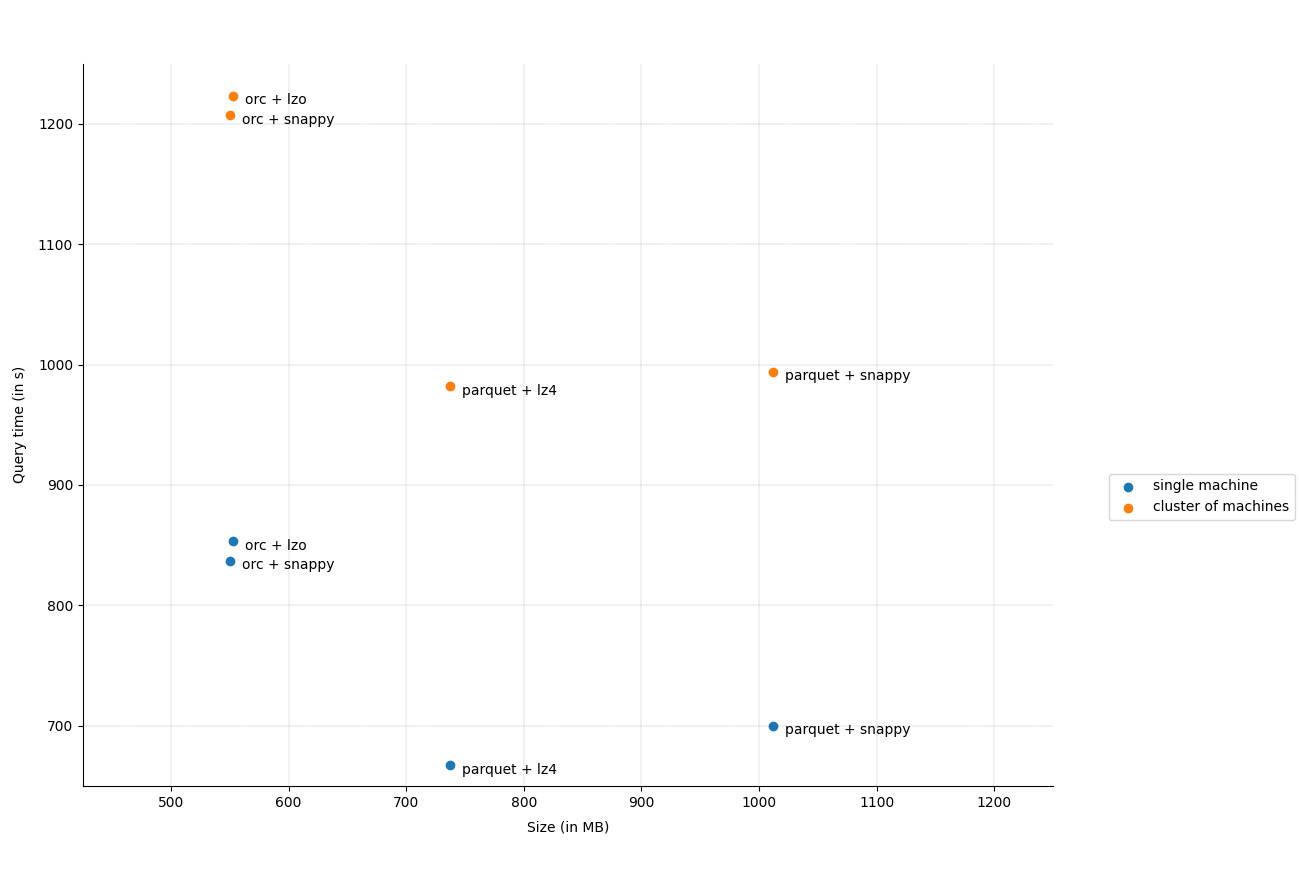
\includegraphics[width=13cm]{./assets/img/comparisons.png}
	\caption{Comparison of results obtained for \textit{lubm1000}}
	\label{fig:result_comparison}
	\vspace{0.5cm}
\end{figure}

\section{Further research}

To extend the reliability of this work, it might be useful to refine the algorithm of translation from SPARQL to SQL presented in Chapter \ref{section:research_methodology} by integrating a reasoner. It might be useful also to test the formats with bigger data sets and different compression algorithms once they would be implemented.

Surely, a following useful experiment might compare the results obtained in this work with those of the systems presented in Chapter \ref{chapter:literature_review} using the same hardware, to find out if the performances are comparable. Following this, if the results were good enough, it might also be useful to compare the obtained performances with other kinds of systems that do not use the schema-free approach as well.

Another experiment might evaluate the four formats tested in this work with other approaches, such as property tables.

% end content

% start acknowledgements

\clearpage
% turn off page numbering
\pagenumbering{gobble}
\chapter*{Acknowledgements}

I would like to express my appreciation and special thanks to my supervisors: Professor Olivier Curé and Professor Marinella Sciortino. The former has sparked (this verb is not a random choice) my interest in the world of Big Data and cloud computing during my semester at Université Gustave Eiffel (France) and guided me throughout the execution of this experiment. The latter has given me the opportunity to be able to realize this ``joint'' thesis and, in addition to this, she has been my mentor during my 5 years at the University of Palermo. I deeply respect both professors on a professional level, not to mention their personal qualities, not so obvious in the academic environment.

I would like to thank Eleonora, who has accompanied me on this journey and helped me to overcome every difficulty.

I would like to thank my family, my colleagues who have become close friends over the years and my lifetime friends.

Last but not least, I would like to thank all the people involved in organizing exchange projects, such as Erasmus\texttt{+} and Project Vinci, which gave me the opportunity to fulfill my lifelong dreams.

% end acknowledgements

% start bibliography
\printbibliography
% end bibliography

\end{document}